% THIS IS AN EXAMPLE DOCUMENT FOR VLDB 2012
% based on ACM SIGPROC-SP.TEX VERSION 2.7
% Modified by  Gerald Weber <gerald@cs.auckland.ac.nz>
% Removed the requirement to include *bbl file in here. (AhmetSacan, Sep2012)
% Fixed the equation on page 3 to prevent line overflow. (AhmetSacan, Sep2012)

\documentclass{vldb}
\usepackage{graphicx}
\graphicspath{ {images/} }
\usepackage{balance}  % for  \balance command ON LAST PAGE  (only there!)
\usepackage{amsmath}
\usepackage{url}
\usepackage{subcaption}
\usepackage{amsmath}
\usepackage[utf8]{inputenc}
\usepackage{booktabs,floatrow}

\usepackage[linesnumbered,ruled]{algorithm2e}
\SetKwRepeat{Do}{do}{while}%

\newcommand{\argmin}{\operatornamewithlimits{argmin}}
\newcommand{\argmax}{\operatornamewithlimits{argmax}}
\newcommand{\para}[1]{\noindent\textbf{#1}}

\begin{document}

% ****************** TITLE ****************************************

\title{ Performance Evaluation of Stream Data Processing Systems}

% possible, but not really needed or used for PVLDB:
%\subtitle{[Extended Abstract]
%\titlenote{A full version of this paper is available as\textit{Author's Guide to Preparing ACM SIG Proceedings Using \LaTeX$2_\epsilon$\ and BibTeX} at \texttt{www.acm.org/eaddress.htm}}}

% ****************** AUTHORS **************************************

% You need the command \numberofauthors to handle the 'placement
% and alignment' of the authors beneath the title.
%
% For aesthetic reasons, we recommend 'three authors at a time'
% i.e. three 'name/affiliation blocks' be placed beneath the title.
%
% NOTE: You are NOT restricted in how many 'rows' of
% "name/affiliations" may appear. We just ask that you restrict
% the number of 'columns' to three.
%
% Because of the available 'opening page real-estate'
% we ask you to refrain from putting more than six authors
% (two rows with three columns) beneath the article title.
% More than six makes the first-page appear very cluttered indeed.
%
% Use the \alignauthor commands to handle the names
% and affiliations for an 'aesthetic maximum' of six authors.
% Add names, affiliations, addresses for
% the seventh etc. author(s) as the argument for the
% \additionalauthors command.
% These 'additional authors' will be output/set for you
% without further effort on your part as the last section in
% the body of your article BEFORE References or any Appendices.

%\numberofauthors{8} %  in this sample file, there are a *total*
% of EIGHT authors. SIX appear on the 'first-page' (for formatting
% reasons) and the remaining two appear in the \additionalauthors section.

%\author{
% You can go ahead and credit any number of authors here,
% e.g. one 'row of three' or two rows (consisting of one row of three
% and a second row of one, two or three).
%
% The command \alignauthor (no curly braces needed) should
% precede each author name, affiliation/snail-mail address and
% e-mail address. Additionally, tag each line of
% affiliation/address with \affaddr, and tag the
% e-mail address with \email.
%
% 1st. author
%\alignauthor
%Ben Trovato\titlenote{Dr.~Trovato insisted his name be first.}\\
%   \affaddr{Institute for Clarity in Documentation}\\
%   \affaddr{1932 Wallamaloo Lane}\\
%   \affaddr{Wallamaloo, New Zealand}\\
%   \email{trovato@corporation.com}
%% 2nd. author
%\alignauthor
%G.K.M. Tobin\titlenote{The secretary disavows
%any knowledge of this author's actions.}\\
%   \affaddr{Institute for Clarity in Documentation}\\
%   \affaddr{P.O. Box 1212}\\
%   \affaddr{Dublin, Ohio 43017-6221}\\
%   \email{webmaster@marysville-ohio.com}
%% 3rd. author
%\alignauthor Lars Th{\Large{\sf{\o}}}rv{$\ddot{\mbox{a}}$}ld\titlenote{This author is the
%one who did all the really hard work.}\\
%   \affaddr{The Th{\large{\sf{\o}}}rv{$\ddot{\mbox{a}}$}ld Group}\\
%   \affaddr{1 Th{\large{\sf{\o}}}rv{$\ddot{\mbox{a}}$}ld Circle}\\
%   \affaddr{Hekla, Iceland}\\
%   \email{larst@affiliation.org}
%\and  % use '\and' if you need 'another row' of author names
%% 4th. author
%\alignauthor Lawrence P. Leipuner\\
%   \affaddr{Brookhaven Laboratories}\\
%   \affaddr{Brookhaven National Lab}\\
%   \affaddr{P.O. Box 5000}\\
%   \email{lleipuner@researchlabs.org}
%% 5th. author
%\alignauthor Sean Fogarty\\
%   \affaddr{NASA Ames Research Center}\\
%   \affaddr{Moffett Field}\\
%   \affaddr{California 94035}\\
%   \email{fogartys@amesres.org}
%% 6th. author
%\alignauthor Charles Palmer\\
%   \affaddr{Palmer Research Laboratories}\\
%   \affaddr{8600 Datapoint Drive}\\
%   \affaddr{San Antonio, Texas 78229}\\
%   \email{cpalmer@prl.com}
%}
% There's nothing stopping you putting the seventh, eighth, etc.
% author on the opening page (as the 'third row') but we ask,
% for aesthetic reasons that you place these 'additional authors'
% in the \additional authors block, viz.

\date{30 July 1999}
% Just remember to make sure that the TOTAL number of authors
% is the number that will appear on the first page PLUS the
% number that will appear in the \additionalauthors section.


\maketitle
\begin{abstract}
Over the last years, stream data processing has been gaining attention both in industry and in academia due to its wide range of applications. To fulfill the need for scalable and efficient stream analytics, numerous open source stream data processing systems (SDPSs) have been developed, with high throughput and low latency being their key performance targets. In this paper, we propose a framework to evaluate the performance of three SDPSs, namely Apache Storm, Apache Spark, and Apache Flink. Our evaluation focuses in particular on measuring the throughput and latency of windowed operations, such as windowed aggregation and join. For this benchmark, we design workloads based on real-life, industrial use-cases. 
The main contribution of this work is threefold. First, we give a definition of latency and throughput for stateful operators. Second, we completely separate the system under test and driver, so that the measurement results are closer to actual system performance under real conditions. Third, we build the first driver to test the actual sustainable performance of a system under test. Our detailed evaluation shows that there is no single winner, but rather, each system shines in individual use-cases.
%All experiments are conducted with maximum and 90\% of the maximum workloads. %Not so interesting here.
%\todo[inline]{Can we also give an indication of the takeaway message here?=>fixed}
\end{abstract}

\section{Introduction}
Stream data processing has been gaining significant attention due to its wide range of uses in big data analytics. The main idea is that processing big volumes of data with batch processing engines is not enough anymore and data has to be processed fast to enable fast adaptation and reaction to changed conditions. Several engines are widely adopted and supported by open source community, such as Apache Storm \cite{toshniwal2014storm}, Apache Spark  \cite{zaharia2012discretized} , Apache Flink \cite{carbone2015apache}. 

One of application areas of stream data processing is  video games. Processing of large scale online data feeds from different sources swift is imperative for online video game companies in industry. For example, once the company releases the new feature of particular video game, fast and efficient analysis of customer usage statistics is a must to determine the their attitudes and satisfaction. In this paper, we collaborate with \textit{Rovio Entertainment}, the video game company. We build the benchmarking system on top of \textit{Rovio} use-case. One use-case is related with analytics on windowed aggregation, calculating the average session time of users within specified geo locations. Another use-case is associated with windowed join, calculating the time lag between clients and company services. 

In this work we propose the benchmarking system to assess the performance of three major, open source and community driven streaming engines, being Apache Storm, Apache Spark and Apache Flink.  Throughout  the tests, we use latency and throughput as the major performance indicators. Latency is the time required to calculate the final result, throughput on the other hand determines the number of successful calculations per unit time. In stream data processing, it is number of tuples per unit time the engine can ingest for further process. We use two \textit{Rovio} use-cases for experiments. 


There are numerous open challenges related with measuring main Key Performance Indicators (KPIs) in stream data processing engines. For example, there is not clear definition for the latency of stateful operator within SDPS.   That is,  the stream is theoretically infinite and there is no final output. While the previous works use checkpointing each event's ingestion and output time, this can lead to misleading results and escalade the driver's complexity. Moreover, while benchmarking SDPSs, it is crucial to separate completely the driver and units under test as otherwise, the results can be biased. Furthermore, the driver should be flexible enough to support different policies to handle system specific features. For example, back-pressure is characteristic feature of SDPSs and while calculating system's sustainability it must be taken into consideration.
Most importantly, keeping the benchmarking system simple while solving the challenges listed above is imperative. 

%\para{Matrix Blocking Through Joins.}
In this paper, we overcome the challenges listed above. The proposed solution is generic, has simple design with clear semantics and can be applied to any SDPS. We keep the design of a solution as simple as possible. The main intuition is to simulate an environment in which we can calculate the KIPs more precisely and with minimum influence of side factors. We design experiments on top of $Rovio$ use-cases.

The main contributions of this paper are listed above:
\begin{itemize}  
\item We first introduce the term sustainability of SDPS and give its definition. The stream data processing engine is sustainable with a given input if it can process it within user-defined quality boundaries.  For example, user can define custom logic which can handle back-pressure while measuring system's sustainability. 
\item  We first  introduce  the mechanism to measure the latency in stateful operators is SDPS. We applied the proposed method with partitioned windowed aggregation and partitioned windowed join use cases. 
\item We accomplish the above contributions with a simple system design in which the KPI measurements are clearly separated from units under test. 
\item We test the proposed benchmark on Storm, Spark and Flink with industry use-cases of $Rovio$.
\end{itemize}

The remainder of paper is organized as follows. In Section \ref{rel}, related benchmarks in stream data processing and in general big data analytics are studied. The preliminary and background information about the engines being tested are analyzed in Section \ref{pre}. The detailed interpretation of open challenges  and their importance are discussed in Section \ref{chal}. We provide the design of benchmark system, the use-cases and KPIs in Section \ref{des}. After evaluations in Section \ref{eval} we conclude in Section \ref{conc}.

\section{Related work}
\label{rel}
%Now with emerging next generation stream data processing engines, batch processing is seen as a special case of stream processing where the data size is bounded. 
Benchmarking distributed data processing systems has been an active area of research. Huang et.al. proposed HiBench \cite{huang2011hibench}, which was the first benchmark suite to evaluate and characterize the performance of  Hadoop. In a more recent version, the benchmark also features a streaming component \cite{white2012hadoop}. The authors conduct a wide range of experiments from micro-benchmarks to machine learning algorithms. A highly related benchmark is SparkBench, which features machine learning, graph computation, SQL queries, and streaming applications on top of Apache Spark \cite{li2015sparkbench}.
Building an application level, end-to-end big data benchmark with all major characteristics in the lifecycle of big data systems  is the main goal of BigBench \cite{ghazal2013bigbench}.
Wang et al. introduce BigDataBench, the big data benchmark suite for Internet services. The BigDataBench suite contains  19 scenarios covering a broad range of applications and diverse and representative data sets \cite{wang2014bigdatabench}.

Benchmarks on SDPSs extend the batch data processing benchmarks and pose unique challenges. Recently, researchers from Yahoo! conducted a series of experiments on stream data processing engines to measure their latency and throughput \cite{chintapalli2016benchmarking}. They used Apache Kafka \cite{kafka2014high} and Redis \cite{carlson2013redis} for data fetching and storage. Later on, on the other hand, it was shown that those systems actually are a bottleneck for the tested systems' performance \cite{dataartisans}. In this paper we overcome this bottleneck and measure event time latency. Marcu et al. did an extensive analysis of the differences between Apache Spark and Apache Flink by correlating the execution plan with  resource utilization and  parameter configuration \cite{marcu2016spark}. The authors conduct experiments with batch and iterative workloads on up to 100 nodes. Their key finding is similar to ours that none of the  systems outperforms the other for all data types, sizes and job patterns. However, the authors leave benchmarking the SDP features of the systems  for the future work, which we present in this paper.

Perera et al. use Karamel \cite{karamel} to provide reproducible batch and SDP benchmarks of Apache Spark and Apache Flink in a cloud environment \cite{perera2016reproducible}.  We can identify the similarity in the results in Spark and Flink's memory usages between that particular work and  our paper. However, for other metrics such as CPU usage and latency, we notice significant differences. The authors used the  Yahoo stream benchmarks for evaluation and  it was shown above that the particular benchmarking framework have bottlenecks; thus, this can be a possible reason for differences in evaluation results. In Section \ref{chal} we analyze this challenge and provide our low-overhead  solution to overcome this bottleneck.
Lopez et al. propose a benchmarking framework to assess the fault tolerance and throughput efficiency for the open source stream data processing engines Storm, Spark and Flink \cite{lopez2016performance}. The key finding of the paper is that  the micro-batch stream processing system, Spark, is more robust to node failures, i.e., it efficiently stores the full processing state of the micro-batches and distributes the interrupted processing with low-overhead among other worker nodes.
On the other hand, Spark performs up to 15 times worse than Storm and Flink. Compared the particular paper with our work,  there are differences in terms of the throughputs of the systems. In our paper, we analyze the \textit{unreal throughput} as being one of the challenges and provide our solution, \textit{sustainable throughput}.   
Shukla et al. perform common IoT tasks with different stream data processing engines, evaluating their performance \cite{shukla2016benchmarking}. 
Firstly, the authors define the latency being an interval  between source operator's ingest and sink operator's emitting time. As we will discuss in Section \ref{chal}, this approach may lead to unrealistic results. Thus, we provide a solution for the event time latency.  Secondly, the authors define throughput  as the  rate of output messages emitted from the sink operators in unit time. However, the output throughput may not be useful in various real-life use-cases. In our paper, we introduce sustainable throughput and provide a low-overhead solution to measure it. 

Lu et al. propose StreamBench, a solution to measure the throughput and latency of a SDSP by putting mediator system between the data source and SUT \cite{lu2014stream}. In Section \ref{chal}, we show that the mediator system can be a bottleneck and resulting benchmarks may not exhibit precise results. Thus, we provide an efficient  solution to use local,  distributed, and efficient mediator system.  The LinearRoad benchmark was proposed by Arasu et al. to measure the performance of standalone stream data management systems such as Aurora \cite{abadi2003aurora} by simulating a toll system scenario for motor vehicle expressways \cite{arasu2004linear}. The authors use response time, which is the time difference between input's arrival and output from SDPS, as a metric. As stated above, this definition of latency can lead to unrealistic results; thus, we provide low-overhead solution to measure event time latency.
Several stream processing systems implement their own benchmarks to measure the system performance without comparing them with any other system \cite{neumeyer2010s4,qian2013timestream,zaharia2012discretized}. 

 \todo[inline]{This is not enough, you should add a differentiation for every or at least every class of related work. This needs to exactly point out, where other the work falls short=>fixed This could still be improved}
%As we overcome the bottlenecks faced in previous works, the resulting system gets simpler, which is one of key points in benchmarking.
 
 

\section{PRELIMINARY AND BACKGROUND}


In this section we provide preliminary and background information about the stream data processing engines used throughout this paper.  Initially, the general information about the working principles of particular system is given.  Afterwards, we provide more use case specific info for each system. Because we test engines' partitioned windowed join and  aggregation operators, basic semantics of particular operators , computational model and back-pressure mechanism are analysed.  
\subsection{Apache Storm}

Apache Storm is a distributed stream processing computation framework which was open sourced after being acquired by Twitter. 


\textbf{Computational model}
Storm operates on tuple streams and provides record-by-record stream processing. It supports at-least-once processing (when there are failures events are replayed) mechanism and guarantees all tuples to be processed. Storm also supports exactly-once semantics with its Trident abstraction. The core of Storm data processing is a computational topology which consists of spouts and bolts.  Spouts are source operators whereas bolts are processing and sink operators. Because Storm topology is DAG structured, where the edges are stream tuples and vertices are operators (bolts and spouts), when a spout or bold emits a tuple, the ones that are subscribed to particular spout or bolt receive input. Storm's parallelism model is based on \textit{tasks}. Each task runs in parallel and by default single thread is allocated per task. 

Storm's lower level API's provide little support for managing the memory and state. Therefore, choosing the right data structure for state management, utilizing memory usage efficiently my making computations incrementally  is up to the user. 
memory management. Storm supports cashing and batching the state transition. However, the efficiency of particular operation degrades as the size of state grows.  Storm  supports back-pressure.



\textbf{Windowing}.
Storm has built-in support for windowed calculations. That is, partitioned windowed joins and aggregations are supported internally.  Although the information of expired, new arrived and total tuples within window is provided through APIs, the state management and making computations incremental  should be done manually. Storm supports processing and event-time windows with sliding and tumbling window features. Processing time windows include time and count based semantics. For event-time windows, tuples should have separate timestamp field so that the engine can create periodic watermarks. One of the downsides of Storm's relying heavily on ackers, is that tuples can be acked once they completely flush out of window. This can be an issue specially, on windows with big length and small slide.  



\subsection{Apache Spark}
Apache Spark is an open source data processing engine, originally developed at the University of California, Berkeley. 

\textbf{Computational model}
Spark internally is batch processing engine. It handles the stream processing by micro-batches. As can be seen from Figure \ref{fig_micro_batch},  Spark Streaming resides at the intersection of batch and stream processing.  Resilient Distributed Dataset (RDD) is a fault tolerant abstraction which enables in memory parallel computation in  distributed cluster environment \cite{zaharia2012resilient}. Unlike Storm and Flink, which support one record at a time, Spark Streaming inherits its architecture from batch processing which support processing records in micro-batches. 

One of Spark's features is that it supports lazy evaluation and tries to  limit the amount of work it has to do. This enables the engine to run more efficiently. Spark also supports DAG based execution graph which works implementing  stage-oriented scheduling. Unlike from Flink and Storm, which also work based on DAG exetuion graph, Spark computing unit in graph is data set rather than streaming tuple and each vertex in graph is a stage rather than operators. RDDs are guaranteed to be processed in order in a single DStream. However, the order guarantee within RDD is not provided since each RDD is processed in parallel. 

Spark Streaming has improved significantly its memory management in recent releases.  The memory is shared between execution and storage. This unified memory management supports dynamic memory management between the two modules. Moreover, Spark supports dynamic memory management throughout the tasks and within operators of each task. 

\textbf{Windowing}
Spark Streaming has a built-in support for windowed calculations. Processing time windows with sliding and tumbling versions are  supported in Spark. The operations done with sliding windows, are internally incrementalized transparent to the user.  However, choosing the length batch interval can affect the window based analytics. Firstly, the latency and response time of windowed analytics is strongly replying on batch interval. Secondly, supporting only processing time windowed analytics, can still be a bottleneck in some use cases. Spark supports back pressure which is very useful in windowed calculations. The window size must be a multiple of the batch interval, because window keeps the particular number of batches until it is purged. 




\subsection{Apache Flink}
Apache Flink which was started off as an academic open source project (Stratosphere \cite{alexandrov2014stratosphere}) in Technical University of  Berlin.

\textbf{Computational model}
Distributed dataflow engine is standing in the core of Flink. It is responsible for executing the dataflow programs. Like Storm, A Flink runtime program is a DAG of stateful operators connected with data streams. Flink's runtime engine supports unified processing of batch (bounded) and stream (unbounded) considering former as being the special case of the latter.

Flink provides its own memory management to avoid long running JVM's garbage collector stalls by serialising data into memory segments. 
The data exchange in distributed environment is done via buffers. So, producer takes a buffer from the pool, fill it up with data, and the consumer receives data and frees the buffer informing the memory manager. There are different mechanisms such as sending when buffer is full or sending when timeout is reached to link buffers between consumer and producer or sending locally or remotely. Flink provides wide range of high level and user friendly APIs to manage the state. The incremental state update, managing the memory or checkpointing with big states is done automatically, transparent to user. 

\textbf{Windowing}
Flink owns strong feature set for building and evaluating windows on data streams. With wide range of pre-defined windowing operators, it supports user defined windows with custom logic. The engine provides processing time, event time and ingestion notion of time.  In processing time, like Spark,  windows are defined with respect to the wall clock of the machine that is responsible for building and processing  a window. In event time on the other hand, the notion of time is  determined when the event are created. Like in Storm, the timestamps must be attached to each event record as a separate field. In ingestion time, the system still processes with event time semantics but on the timestamps which were assigned when tuples arrive the system. Flink has a support for out-of-ordered streams which gained popularity after Googles MilWheel and Dataflow papers \cite{akidau2013millwheel,akidau2015dataflow}

\section{Challenges}
\label{chal}
There are several challenges to be taken into consideration while designing a benchmark for SDPSs. In this section we analyse the challenges and provide solutions.

\para{ \textit{Simple is beautiful}}. The first challenge is to design a simple system for the driver, because this avoids extra overheads and bottlenecks and of course, simple is beautiful. As the number of sub-systems included in driver increases, the complexity escalades at the same time. One of downsides of the complex system is, difficult to determine the bottleneck. One example is the connection system between data generator and SUT.  To test the stream data processing engine, the data generator component is essential, to simulate the real life scenarios. Figure \ref{fig_queue_link} shows possible three cases to link data generator and SUT. The simplest design would be connecting the SDPS directly to data generators as shown in Figure \ref{fig_no_queue}. Although this is perfectly acceptable case, it confronts with real life use cases. That is,  in real life, the stream data processing engines, do not connect to pull based data sources unless there is a specific system design. Usually, SDPSs pull data from the distributed message queues which reside between data sources and SUT as shown in Figure \ref{fig_yes_queue}. One bottleneck of this option is throughput which is bounded by the maximum throughput of message queueing system. Moreover, there is another  de-/serialization layer  which \textit{artificially} increases SUT's latency. We selected the third option which stands between the first two. As can be seen from Figure \ref{fig_partial_queue}, we embedded the queues as a separate module in data generators. In this way, the throughput is bounded only by network bandwidth, the system works more efficiently as there are no de-/serialisation overheads, it can scale out easily and finally it has a simple design. 


\para{ \textit{Isolate driver and test units}}. The second challenge is to isolate the benchmark driver and SUT as much as possible. For example, in SDPSs benchmarks, it is common to measure the throughput inside the SUT. Because both computations (driver and test) can affect each other the results can be  biased  which is discussed below. We solved this problem by categorising the test unit and pointing measurements accordingly. The first evaluation is throughput. Throughput is associated with the system. So, we kept the throughput assessment outside the SUT, inside data generator module. The second evaluation is latency. The latency is linked with an operator inside system. So, we kept all latency measurements outside the particular operator.

\para{ \textit{ Artificial latency and throughout}}.
The third challenge is to abstain from biased test results and keep the evaluation semantics clear.  One example for this is, throughput measurement. In the previous SDPS benchmarks, the throughput of a SUT is measured by either taking quantiles over test time, or showing max, min and average assessments. From user's perspective on the other hand, the system's maximum throughput is  defined as upper bound  for processing the given workload. When conducting the experiments with stream data processing engines, back pressure is one factor affecting the throughput, that should be taken into consideration.  We solve the first issue by measuring the SUT's max throughput with maximum workload that it can sustain. We give the definition of SUT's sustainability with given workload.
The mechanism we provide for measuring sustainability is customisable based on user's preferences. For example, it can take user-defined function and measure sustainability according to particular function. In this way, we can easily plug the custom logic for back-pressure handling. 

 Another example for this challenge is latency measurement. Latency is a time interval between the stimulation and response. For batch data processing systems, we assume that data is already in the system so, the latency is the interval between tuples' read and output. For SDPSs on the other hand, the latency is the time between tuple's event time and output. If there are extra systems between SDPS and data source, then those are likely to add \textit{artificial latency} for each tuple.  Some researchers circumvented this problem by measuring latency in SDPS the same as in batch data processing systems. In this case, the number and complexity of the systems between SDPS and data source is regardless as latency is the interval between tuples' ingestion and output. However, this measure of latency is \textit{optimistic} as latency for SDPSs is between tuple's event time and output time. Another factor triggering the \textit{artificial latency} is input data rate. If the input data rate is higher than the SDPS can sustain, the results can be biased. Even if the system supports back-pressure, if data rate is more than it can sustain, initially the system will try to ingest as much data as possible. Then, the calculation time will take longer and the latency will increase for every tuple. For this case, it is crucial to measure system's sustainability rate and calculate the latency in that specific configuration, otherwise the measurements will be biased.  We solve this issue by clearing the systems creating artificial latency between data source and SDPS and measuring the latency with the sustainable throughput only. 
 


\para{ \textit{ Latency of stateful operator}} The fourth challenge is measuring the latency of stateful operator. Up to this point, the related works in the literature either concentrated on stateless operators or evaluated the latency of stateful operators by checkpointing to external systems like lightweight distributed databases. As we discussed above, this approach can be a bottleneck in some cases. In this paper, we  define the latency of stateful operator formally and  provide a solution for this problem without any external system. Basically, the latency of the target operator can be calculated by just putting extra operator adjacent to it and the difference in tuple's timestamp and current timestamps are calculated in particular operator.

\begin{figure*}
    \centering
    \begin{subfigure}[b]{0.32\textwidth}
        \includegraphics[width=\textwidth]{eps/no_queue}
        \caption{Without message queue}
        \label{fig_no_queue}
    \end{subfigure}
    ~ %add desired spacing between images, e. g. ~, \quad, \qquad, \hfill etc. 
      %(or a blank line to force the subfigure onto a new line)
    \begin{subfigure}[b]{0.32\textwidth}
        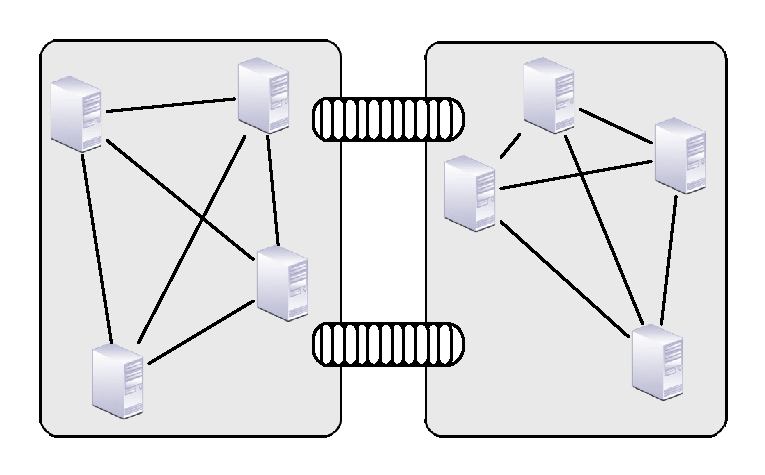
\includegraphics[width=\textwidth]{eps/yes_queue}
        \caption{With message queue}
        \label{fig_yes_queue}
    \end{subfigure}
    \begin{subfigure}[b]{0.32\textwidth}
        \includegraphics[width=\textwidth]{eps/node_queue}
        \caption{Partial message queue}
        \label{fig_partial_queue}
    \end{subfigure}
        \caption{Different system designs to link data generator and SUT.}
            \label{fig_queue_link}
\end{figure*}

\section{Benchmarking framework design}
\label{des}
We discuss the design of the benchmarking framework in this section. As shown in Figure \ref{fig_design}, there are two main components of test deployment: \textit{1)} the SUT and \textit{2)} the driver. The driver has two subcomponents being \textit{i)} Data Generator and \textit{ii)} Data Queue.


\begin{figure}[h]
\centering
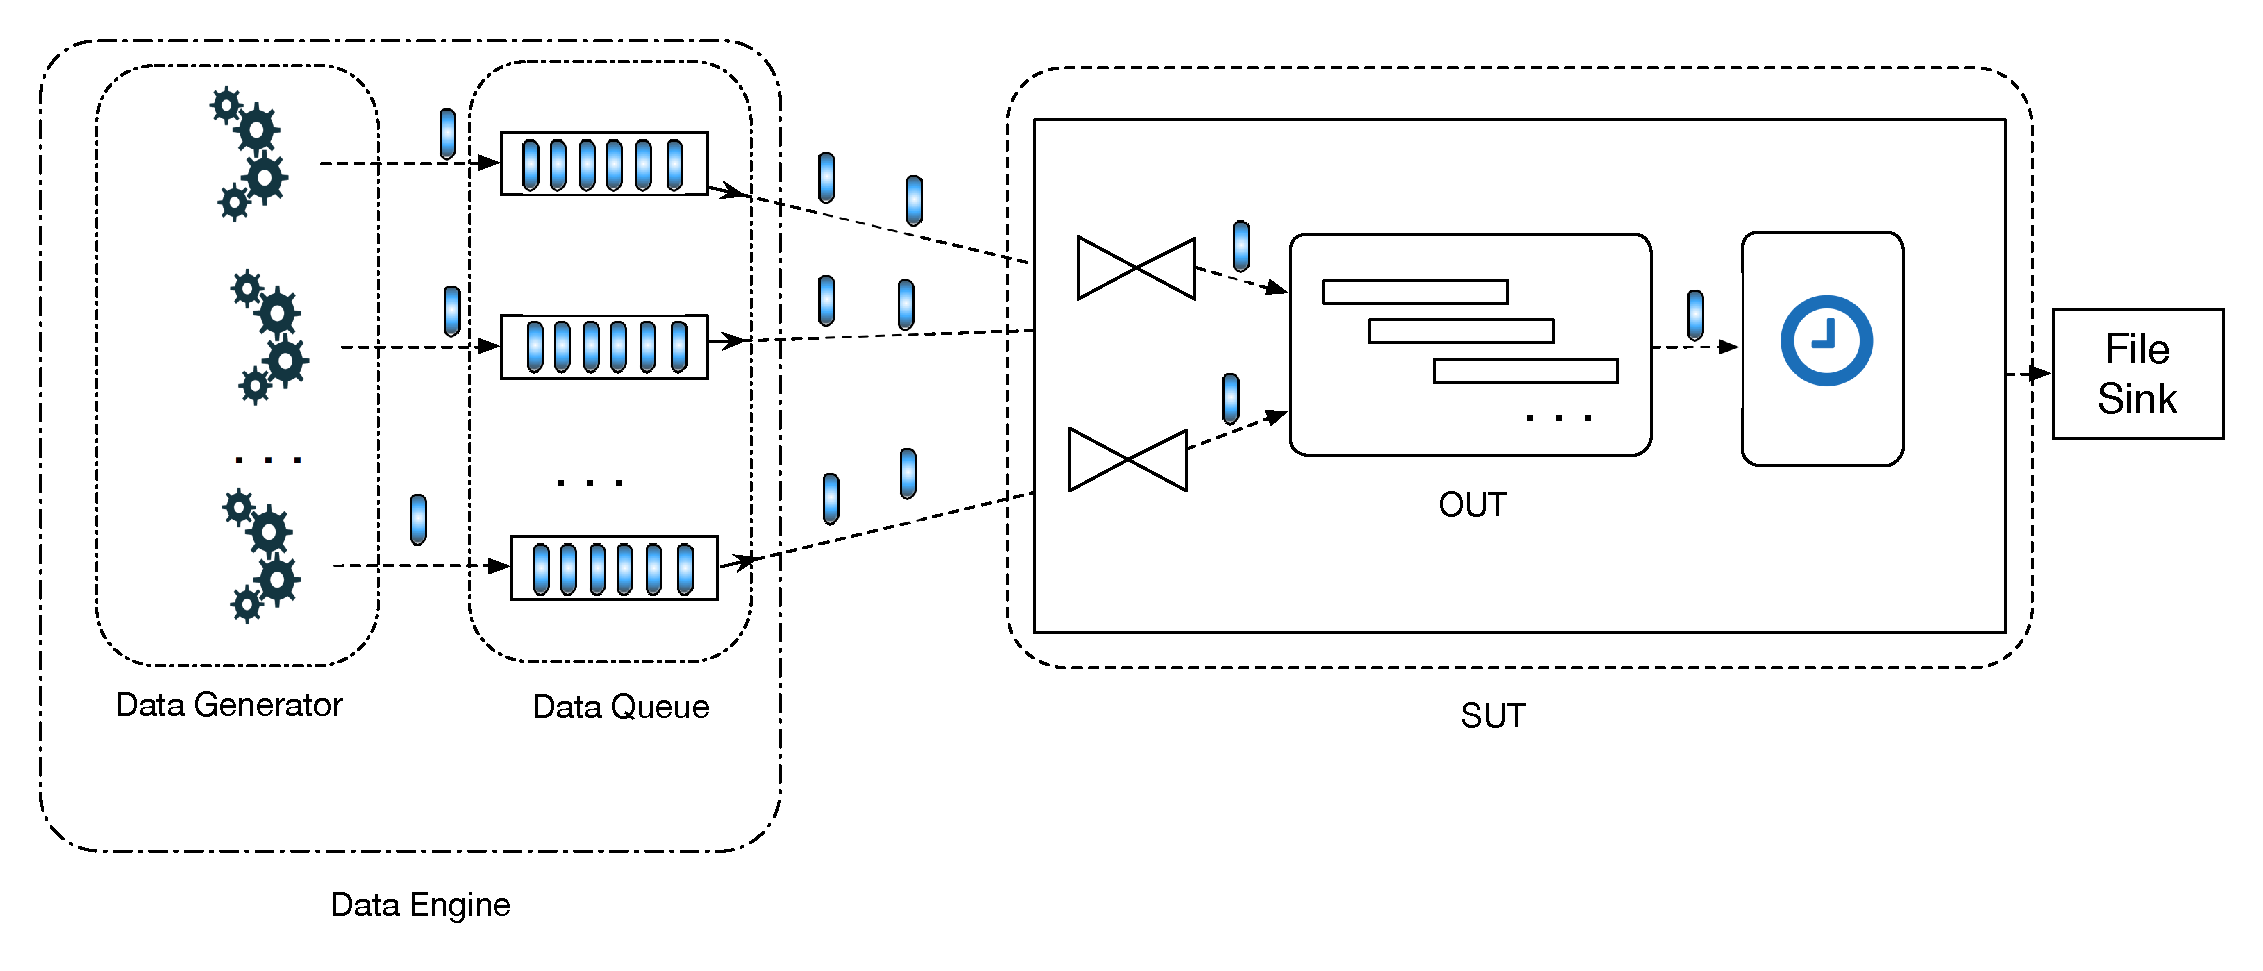
\includegraphics[width=\columnwidth]{eps/system_design}
\caption{Design of the benchmark framework.}
\label{fig_design}
\end{figure}


The Driver Instance (DI) is a combination of the Data Generator Instance (DGI) and the Data Queue Instance (DQI). %\todo[inline]{What is a slot in this setup? Please introduce the general cluster setup=>fixed} 
The driver is the combination of all DIs. Similarly, the Data Generator Subcomponent (DGS) and Data Queue Subcomponent (DQS) are the combination of all DGIs and DQIs, respectively. The driver is responsible for generating and queuing the data. It is composed of finite number of instances which are distributed evenly to the worker nodes in the cluster. The driver nodes are separate from SUT nodes in the cluster deployment. %\todo[inline]{on the same nodes as the SDPS?=>fixed}
The DGI and the DQI reside in the same machine to avoid any network overhead and to ensure data locality. The data is kept in memory to avoid disk write/read overhead. The first subcomponent, the DGS, generates data with a constant speed. Because of the bottlenecks explained in Section \ref{chal}, we avoid using mediator data queueing systems between the driver and SUT but use distributed local queues (DQS). Data is queued in first-in/first-out manner in the DQS. As explained earlier, this approach is not different from implementing centralized and distributed message queues between the SUT and the driver. The following analogy can be made: the queue topic   in a distributed message queuing system is analogous to DQS, and the queue partition is analogous to DQI. 
%\todo[inline]{A topic is not a queue, again, please be precise=>fixed}

The data generator  timestamps every event. The event's latency is calculated from this point and the longer it stays in a  queue, the higher its  latency. The number of DIs can be arbitrary and the overall throughput that can be generated is only bounded by the network bandwidth.%\todo[inline]{what is it?, the DI or the DC?=>DI is single driver instance. We dont have a bound on the number of DIs}
% \todo[inline]{How is it measured?=>explained in challenges section}

%\todo[inline]{what do you mean by outer world?=>deleted}
%\todo[inline]{Can any of the systems work with push-based sources?=>for example we could create data inside the system's source operator. This can be push based. Anyway , I deleted the  sentence.}
%. \todo[inline]{This is hard to understand, also explaining all the separation without actually explaining the measurement is confusing and from a structure point of view not good. Most of this, you already said in the challenges section. It is probably best to shorten this to the architecture part.=>deleted whole paragraph}


%Proper handling tuples' timestamp fields while joining or aggregating is crucial. In this work, \textit{merging} of tuples' timestamp fields is done by selecting \textit{maximum} over them. That is, latest arrived tuple's timestamp is transferred to the new tuple as a result of aggregation or join. Equation \ref{eq_1} defines this logic formally.
%
%
%Here $t \in T$ is a stream tuple,  $t[k]$ is  $k^{th}$ field of particular data point and $\equiv$ means equivalent in terms of type. For aggregation function $|T|$, the size of a set is not bounded, whereas for join function it is bounded by two, being $|T| = 2$.



The use-cases for this benchmark are derived from an online video game applications. Online video game companies continuously monitor the user actions in a game and ensure that the system works as expected. For example, the company tracks the number of active users and take actions on a sudden drop. Moreover, once the new feature is added to an online game or the game is updated to a new version, the company monitors the application to see  the newly added feature is working  without failures.
%\todo[inline]{Maybe change this to the use case Henri provided=>fixed}

%\textbf{Windowed Aggregation}
Windowed aggregations are an important part of the user monitoring in online video gaming. Online video game companies track the IAPs per application, per distribution channel(the application store, e.g. iTunes/appStore, Google Play), per product item (the actual IAP item like gem pack) and etc. In this benchmark, we use similar use-case monitoring the IAPs per product item. 
%\todo[inline]{Please adjust according to Henri's feedback->fixed}

%\textbf{Windowed Join}
Windowed joins are another important part of user monitoring in online video gaming.  Analysing the IAPs within a game and comparing the results based on distribution channel, user ID, and etc. is another use-case in online video game industry. In our benchmark, we get user feeds per distribution channel and compare the IAPs of the same product item between streams. That is, we divide the input streams into windows and join them per key (product item). 
%\todo[inline]{Again the same sentence as above=>fixed}
%\todo[inline]{is this relevant for us?=>fixed}


\subsection{Metrics}
The metrics for this benchmark are latency and throughput. In this section, we give the definition of each metric and explain our solution to measure it. 


%To measure the performance of a system, we connected max $16$ data generators to system under test with order of $1$,$2$,$4$,$8$ and $16$ as increasing further does not increase the overall throughput significantly. We call the tests with related workloads as $1x$, $2x$, $4x$, $8x$ and $16x$. Moreover, the configuration of each data generator must be the same. Configuration includes parameters such as overall input size, generation speed, socket port and etc. Equation \ref{eq_2} defines this formally.
%
%\begin{equation}
%  \begin{gathered}
% \textbf{Let} \ d_{i}^{c_{i}} \in  D\\
%  \textbf{then}, |D| \gets S \\
%  \textbf{and} \ c_{1} = c_{2} \ ... = c_{n}, \forall n \in S = {1,2,4,8,16}
%  \end{gathered}\label{eq_2}
%\end{equation}


\subsubsection{Throughput}

As we defined above, we use the maximum sustainable throughput to measure system's workload. Throughout the experiments, the data generation speed in all DIs are equal and constant. To examine if a system can sustain a given throughput, we divide the queue used in DQI into three parts: $q^{a}$ , $q^{b}$ and $q^{n}$. Figure \ref{fig_queue}, shows the example partitioning of the queue. If the size of the queue is less than or equal to $c^{a}$ throughout the experiment, then this is acceptable, meaning the SUT can sustain the given throughput. If the queue size is between $q^{a}$ and  $q^{b}$ on the other hand, the SUT cannot sustain the given data rate, but the driver might tolerate it for some time. A longer queue can be caused by slow system initialization, backpressure, etc. However, if the queue size is longer than $q^{b}$ then the SUT cannot sustain the given throughput and the latency is expected to continuously increase. In this case we end the experiment.

% \todo[inline]{You repeat yourself here, without explaining the sustainable throughput and the maximum throughput. Please start by explaining these before saying they are different. Probably this paragraph can be deleted completely.=>deleted all of them}

\begin{figure}[h]
\centering
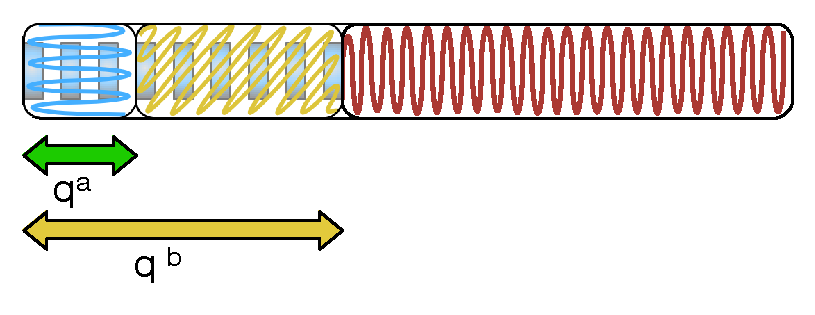
\includegraphics[width=0.5\textwidth]{eps/queue}
\caption{Basic intuition behind \textit{backpressure-compatible queue}}
\label{fig_queue}
\end{figure}
%\todo[inline]{Is this figure ever referenced in the text?=>yes}


\begin{lstlisting}[
language=SQL,
showspaces=false,
basicstyle=\ttfamily,
numbers=left,
numberstyle=\tiny,
commentstyle=\color{gray}
label={lst:label},
caption={Queries},
captionpos=b
]
S_1 = UNION  {s_1, s_2, ..., s_m}
S_2 = UNION {s_m, s_m+1, ..., s_n}
S_3 = UNION  {s_1, s_2, ..., s_n}

Query_1 = SELECT AVG(S_1.price)
FROM S_1 on window(l, s) 
GROUPBY S_1.geo

Query_2 = SELECT MAX(S_2.price, S_3.price)
FROM S_2, S_3 on window(l, s) , 
WHERE S_2.geo = S3.geo and S_2.ts = S3.ts

Query_3 = 
1.UPDATE S_1, S2: enrich with a new field = 
   cnt,  the country name of geo location
2.SELECT AVG(R.price)
  FROM  
   (SELECT MAX(S_2.price, S_3.price)
    FROM S_2, S_3 on window(l, s), 
    WHERE S_2.cnt = S3.cnt and S_2.ts = S3.ts)  
    as R on window(l, s)  
  GROUPBY R.geo
  WHERE R.price > 100




\end{lstlisting}

%The semantics behind the evaluation of a sustainable workload with a given throughput must be clear. Moreover, it should support the system specific behaviors like backpressure. 
Our system supports user-defined policies to test the sustainability. For example, one policy tolerates the $q^{b}$ part of the queue for a given time period (time based policy). Another policy tolerates   the $q^{b}$ part of the queue for a given number of pushes into the queue (count based policy).% \todo[inline]{not sure what this means=>fixed}
This policy is customizable and can be easily plugged into the driver. %\todo[inline]{DEC?=>fixed}  



We choose a policy that is a combination of time and count based policies. Once the queue size exceeds the $q^{a}$ and is less than $q^{b}$, we wait until $\frac{q^{b} - q^{a}}{2}  $ elements are pushed into the queue and check again. If the queue size is still bigger than $c^{a}$ we end the benchmark concluding the SUT cannot sustain the given throughput. %If the queue size is within $c^{a}$ and $c^{b}$, we do not tolerate it anymore. 
This process is done continuously in all DIs %\todo[inline]{DEI?=>fixed} 
and if the SUT fails to sustain one instance of the driver, then the experiments are halted meaning the SUT cannot sustain the given throughput. That is, the SUT can sustain a given workload if it can sustain the throughput of all DIs.%\todo[inline]{DEI?=>fixed}  

\textcolor{red}{ It is crucial that separation of driver and SUT and handling backpressure in the driver side does not cause side effects in metric measurements. To emplasize again, the driver does not stop the benchmark when the system exhibits backpressure. Firstly, accurate selection of $q^{a}$, $q^{b}$ and $q^{n}$ is crucial. In our experiments, first we assign 5\%, 15\% and 30\% of input size for variables $q^{a}$, $q^{b}$ and $q^{n}$ respectively. In this case, the system can "handle" the given input; however, with longer experiments it fails, as the size of the queue keeps increasing. Moreover, we get very big latencies for the given input. As a result, we keep decreasing the variables until we find the best thresholds for all systems.    Secondly, it is crucial for the driver to distinguish unsustainable throughput and backpressure. As we discussed in above paragraph, the driver can successfully handle this issue. If the queue size gets beyond $q^{a}$ and less than $q^{b}$, the driver starts to inspect the queue for the next $\frac{q^{b} - q^{a}}{2}  $ tuples. If the queue size keeps increasing, for every such tuple, then we conclude that this is not a backpressure. In fact in experiments, we show that our driver can successfully handle the backpressure.}







\subsubsection{Latency}
\label{sec_latency}
%Latency is another metric for this benchmark and  the defining of latency also needs clear semantics. There are several points that need to be clarified: \textit{i)} the aggregation or join of timestamp fields of tuples and \textit{ii)} the period  (start and end time) of latency.

%The first point is the aggregation or join of tuples with timestamp fields. 
While the use-case provides the semantics for aggregating or joining tuples, the semantics for measuring the latency of stateful operators is unclear.  We provide efficient solution for this problem in our benchmarking framework. When the tuples arrive to a stateful operator, it does the aggregation that is defined in the use-case. Besides the aggregation  defined in the use-case,  we aggregate the timestamp fields of tuples within stateful operator. That is, the timestamp of stateful operator's output tuple is the maximum timestamp of all tuples inside the operator.  The main intuition is that we exclude the tuples' waiting time in the window by taking the timestamp of the latest arrived tuple in each window. When a record is emitted from the sink operator of the SUT, we calculate the latency of a tuple by subtracting its timestamp from the current time.



\textcolor{red}{ We are aware of the fact that new definition of latency can be applied when the data is pushed to the system. }
%\todo[inline]{You define many variables here, but do not really use them. Maybe an intuitive explanation would be better.=>fixed}


%\todo[inline]{after reading this, I don't clearly understand how you measure / calculate the latency and where this is done.=>deleted}






\section{Evaluation}
\label{eval}
In this section, we discuss our experimental results. We run experiments in 2-, 4-, and 8-node clusters to measure the scale out feature of the systems under test. Throughout the experiments we used Storm 1.0.2, Spark 2.0.1 and Flink 1.1.3.  The experiments are done with the maximum and 90\% sustainable throughputs. Throughout the experiments, each DI generates 100M events and we use 16 parallel DIs in the cluster. 
%\todo[inline]{Why does a DI have an *input* size? Do you mean the total number of records generated?->fixed} 
We allocate 16 CPUs and 16GB RAM for every node. %\todo[inline]{what does this mean? what does a server have per node? and what engine do you mean?=>fixed} 
All nodes' system clocks in the cluster are synchronized via an NTP server. We generate events with normal distribution.\todo[inline]{what does it mean normla distribution here? With respect to which field?} The network bandwidth is 1Gb/s. We only use processing time windows in the experiments as it is the only window type that all three systems support. We conducted experiments with event time windows with Storm and Flink; however, the results were very similar to the experiments with processing time windows; therefore, we provide only latter in this paper. 
%\todo[inline]{actually, maybe it would be interesting to add event time windows for Storm and Flink=>currently we cannot do it, because of time limitation}. 
We select $q^{a}$ to be 5\% and $q^{b}$ 10 \% of the overall input. Although we did experiments with lower values of the particular variables, it was hard to detect the systems' maximum sustainable throughput. The reason is that  the systems under test use pull-based mechanism to get data from DQS and and the smaller the queue size the more difficult to test SUT's upper limit workload.  We use approximately 25\% of the input data as a warmup. So, in all experiments we exclude the first 25\% of output. The backpressure is enabled in all systems to ensure the durability of experiments. That is, we do not want the systems to ingest more input than they can process and crash during the experiment. In preliminary experiments, measuring the maximum throughput without backpressure mechanisms lead to various exceptions. If the SUT drops one or more connections to the DI, then the experiment is halted with the conclusion that the SUT cannot sustain the given throughput. Similarly, in real-life if the system cannot sustain the user feed and drops connection, then this is considered as a failure.  


Tuning the engines' configuration parameters is important to get a good performance for the given use-cases. %\todo[inline]{what are aggregation partitioned windows?=>fixed}
There are several properties for each SDPS, that need to be tuned to customize the given use-case. For example, in Flink the buffer size has to be adjusted properly to ensure a good balance between throughput and latency. Although selecting low buffer sizes can result in low system latency, the actual latency of tuples may increase as they will be queued in the DQI instead of the buffers inside the system. In Spark the block interval for partitioning the RDDs is one key aspect to tune the system for the given use-case. The number of RDD partitions a single mini-batch  is bounded by $batchInterval \ / \ blockInterval$. As the cluster size increases, decreasing the block interval can increase the parallelism. One of the main reasons that Spark scales up very well is the partitioning of RDDs. However, depending on the use-case, the optimal number of RDD partitions can change. In Storm the number of workers, executors and buffer size are the the configurations (among many other) that needs to be tuned to get the best performance. Similar to Flink, choosing the buffer size is a key to balance between latency and throughput. For all systems,  choosing the right parallelism level is essential to balance between a good resource utilization and network or resource exhaustion.
%\todo[inline]{can you comment on the parameters that you set and how you determined the right parameters? This would be more helpful then just saying that this needs to be done=>below}




\subsection{Keyed Windowed Aggregations}

In the first use-case, we use parti\-tioned  windowed aggregations in Storm, Spark, and Flink. We calculate the maximum sustainable  throughput for  each SDPS. To confirm that the engines are saturated, we performed the same experiments with 90\% of the maximum throughput. We calculate the latency measurements for each system over the respective throughputs.  

    \begin{table*}
        \resizebox{\textwidth}{!} {\begin{tabular}{lllll}\toprule
            &\textbf{2-node}  & \textbf{4-node} & \textbf{8-node}\\\midrule
            Storm & 1407, 66, 5758, (2330, 2721, 3477) & 2058, 115, 12216, (3724, 5856, 7767) & 2253, 179, 17762, (3818, 6467, 9245) \\
            Storm(90\%) & 1100, 84, 5752, (1832, 2176, 2859) & 1676, 43, 9280, (2985, 4140, 6330) & 1932, 182, 11040, (3324, 5005, 7630) \\
            Spark & 3673, 2537, 8596, (4603, 4953, 5990) & 3394, 1987, 6994, (4076, 4315, 4955) & 3139, 1223, 6946, (3896, 4162, 4711)\\
            Spark(90\%) & 3416, 2354, 8005, (3936, 4550, 5443) & 2822, 1630, 6925, (3473, 3767, 4804) & 2781, 1702, 5961, (3624, 3948, 4834)\\
            Flink & 563, 4, 12328, (1448, 2282, 5233) & 265, 4, 5132, (612, 1242, 2479) & 258, 4, 5469, (574, 1228, 3975) \\
            Flink(90\%) & 310, 3, 5826, (698, 1185, 2009) & 250, 4, 5112, (601, 1334, 2430)  & 219, 2, 5405, (482, 843, 3458) \\
        \end{tabular}}
        \caption{ Latency statistics, avg, min, max, and quantiles (90, 95, 99) in milliseconds for windowed aggregations. \todo[inline]{This should be transformed to an actual table with named columns for the metrics (I know it's difficult but it can be done.)}}
         \label{tab_lat_agg}
    \end{table*} 



    \begin{table}
        \begin{tabular}{lllll}\toprule
            &\textbf{2-node}  & \textbf{4-node} & \textbf{8-node}\\\midrule
            Storm & 408K & 696K & 992K  \\
            Spark & 379K & 642K & 912K  \\
            Flink & 1230K & 1260K & 1260K  \\
        \end{tabular}
        \caption{Sustainable throughput for windowed aggregations. }
        \label{tab_th_agg}
    \end{table} 


%\usepgfplotslibrary{statistics}
\pgfplotsset{compat=1.8}
\usetikzlibrary{pgfplots.statistics}
\makeatletter
\newcommand*\bigcdot{\mathpalette\bigcdot@{1.2}}
\newcommand*\bigcdot@[2]{\mathbin{\vcenter{\hbox{\scalebox{#2}{$\m@th#1\bullet$}}}}}
\makeatother


\makeatletter
\newenvironment{customlegend}[1][]{%
    \begingroup
    % inits/clears the lists (which might be populated from previous
    % axes):
    \pgfplots@init@cleared@structures
    \pgfplotsset{#1}%
}{%
    % draws the legend:
    \pgfplots@createlegend
    \endgroup
}%

% makes \addlegendimage available (typically only available within an
% axis environment):
\def\addlegendimage{\pgfplots@addlegendimage}
\makeatother



\begin{figure}

\begin{tikzpicture}

\begin{axis}[
scaled y ticks = false,
legend entries={simulation,
                measurement,
                sample 1}, 
                legend style={at={(axis cs:6.0,0.84)},anchor=south west},
boxplot/draw direction=y,
ylabel={Latency (millisecond)},
height=4cm,
boxplot={
    %
    % Idea: 
    %  place the 
    %  group 1 at 0.3333 and 0.6666
    %  group 2 at 1.3333 and 1.6666
    %  group 3 at 2.3333 and 2.6666
    %  ...
    % in a formular:
    draw position={1/4 + floor(\plotnumofactualtype/3) + 1/5*mod(\plotnumofactualtype,3)},
    %
    % that means the box extend must be at most 0.33333 :
    box extend=0.1,
},
% ... it also means that 1 unit in x controls the width:
x=1cm,
% ... and it means that we should describe intervals:
xtick={0,1,2,...,10},
ytick={0, 500,10000},
x tick label as interval,
xticklabels={%
    {\tiny 2-node \\ max th.},%
    {\tiny 2-node \\ 90 \% th.},%
    {\tiny 4-node \\ max th.},%
    {\tiny 4-node \\ 90 \% th.},%
    {\tiny 8-node \\ max th.},%
    {\tiny 8-node \\ 90 \% th.},%
},
    x tick label style={
        text width=4.5cm,
        align=center
    },
]
\addlegendimage{line legend,green}
\addlegendentry{ \textcolor{red}{\scriptsize{Storm}   }  }
\addlegendimage{line legend,blue}
\addlegendentry{\textcolor{blue}{\scriptsize{Spark}}}
\addlegendimage{line legend,blue}
\addlegendentry{\textcolor{black}{\scriptsize{Flink}}}
    % 2 node 100
\addplot[color=red,
    boxplot prepared={
      average=1407,
      lower whisker=66,
      upper whisker=5758,
      lower quartile=168,
      upper quartile=3477,
      median=1100
    },
    ] coordinates {};
    
\addplot[color=blue,
    boxplot prepared={
      average=3673,
      lower whisker=2537,
      upper whisker=8596,
      lower quartile=340,
      upper quartile=5990,
      median=2578
    },
    ] coordinates {};
    
    
\addplot[color=black,
    boxplot prepared={
      average=563,
      lower whisker=4,
      upper whisker=12328,
      lower quartile=15,
      upper quartile=5233,
      median=161
    },
    ] coordinates {};
    % 2 node 90
\addplot[color=red,
    boxplot prepared={
      median=1,
      upper quartile=1.2,
      lower quartile=0.4,
      upper whisker=1.5,
      lower whisker=0.2
    },
    ] coordinates {};
    
    
\addplot[color=blue,
    boxplot prepared={
      median=1,
      upper quartile=1.2,
      lower quartile=0.4,
      upper whisker=1.5,
      lower whisker=0.2
    },
    ] coordinates {};
\addplot[color=black,
    boxplot prepared={
      median=1,
      upper quartile=1.2,
      lower quartile=0.4,
      upper whisker=1.5,
      lower whisker=0.2
    },
    ] coordinates {};
    
        % 4 node 100
    \addplot[color=red,
    boxplot prepared={
      median=1,
      upper quartile=1.2,
      lower quartile=0.4,
      upper whisker=1.5,
      lower whisker=0.2
    },
    ] coordinates {};
    
    
\addplot[color=blue,
    boxplot prepared={
      median=1,
      upper quartile=1.2,
      lower quartile=0.4,
      upper whisker=1.5,
      lower whisker=0.2
    },
    ] coordinates {};
\addplot[color=black,
    boxplot prepared={
      median=1,
      upper quartile=1.2,
      lower quartile=0.4,
      upper whisker=1.5,
      lower whisker=0.2
    },
    ] coordinates {};
    
            % 4 node 90
    \addplot[color=red,
    boxplot prepared={
      median=1,
      upper quartile=1.2,
      lower quartile=0.4,
      upper whisker=1.5,
      lower whisker=0.2
    },
    ] coordinates {};
    
    
\addplot[color=blue,
    boxplot prepared={
      median=1,
      upper quartile=1.2,
      lower quartile=0.4,
      upper whisker=1.5,
      lower whisker=0.2
    },
    ] coordinates {};
\addplot[color=black,
    boxplot prepared={
      median=1,
      upper quartile=1.2,
      lower quartile=0.4,
      upper whisker=1.5,
      lower whisker=0.2
    },
    ] coordinates {};

            
            % 8 node 100
\addplot[color=red,
    boxplot prepared={
      median=1,
      upper quartile=1.2,
      lower quartile=0.4,
      upper whisker=1.5,
      lower whisker=0.2
    },
    ] coordinates {};
    
    
\addplot[color=blue,
    boxplot prepared={
      median=1,
      upper quartile=1.2,
      lower quartile=0.4,
      upper whisker=1.5,
      lower whisker=0.2
    },
    ] coordinates {};
\addplot[color=black,
    boxplot prepared={
      median=1,
      upper quartile=1.2,
      lower quartile=0.4,
      upper whisker=1.5,
      lower whisker=0.2
    },
    ] coordinates {};

            
            
             % 8 node 90
 \addplot[color=red,
    boxplot prepared={
      median=1,
      upper quartile=1.2,
      lower quartile=0.4,
      upper whisker=1.5,
      lower whisker=0.2,
       average = 4.05
    },
    ] coordinates {};
    
    
\addplot[color=blue,
    boxplot prepared={
      median=1,
      upper quartile=1.2,
      lower quartile=0.4,
      upper whisker=1.5,
      lower whisker=0.2
    },
    ] coordinates {};
\addplot[color=black,
    boxplot prepared={
      median=1,
      upper quartile=1.2,
      lower quartile=0.4,
      upper whisker=1.5,
      lower whisker=0.2
    },
    ] coordinates {};


\end{axis}

\end{tikzpicture}
\caption{dede}
\end{figure}


The maximum sustainable throughput of the SDPSs are shown in Table \ref{tab_th_agg}. We use a four second batch-size for  Spark, as it can sustain the  maximum throughput with this configuration. We identified that for 4- and 8-node configurations, Flink's performance is bounded by network bandwidth.  Storm's and Spark's performance in terms of throughput are comparable, with Storm outperforming Spark by approximately 8\% in all configurations. One reason for Spark's worse performance can be the  overhead of starting periodic  mini-batch jobs. %\todo[inline]{do not understand->fixed}
Storm and Flink, on the other hand, are operating on tuples and, therefore, can sustain higher sustainable throughputs. % \todo[inline]{That is unintuitive, generally, batch systems have higher throughput but also higher latency->changed throughputs to sustainable throughputs}
 We want to stress that the sustainable throughput is not the same as an engine's peak throughput. %  \todo[inline]{Why is the mini batch architecture reason for that?=>deleted}
 As stated above, we are interested in measuring maximum sustainable  throughputs of SUTs in this paper.  We adjusted Spark's block interval to achieve a better parallelism on RDD level and the highest sustainable throughput. Storm introduced  backpressure feature in recent releases; however, it is not mature yet. With high workloads, it is possible that the backpressure stalls the topology, causing spouts to stop emitting tuples. Moreover, we notice that Storm  drops some connections to the DIs when tested with high workloads with backpressure disabled, which is not acceptable according to the real world use-cases. Dropping connections due to high throughput is considered  a system failure.


Table \ref{tab_lat_agg} shows the latency measurements of windowed aggregations. We conduct experiments with the maximum and 90\%-workloads and report $avg$, $min$, $max$, and  quantiles (90,95,99) over the results. %\todo[inline]{fix quantiles->fixed} 
 The latencies shown in this table are computed with the workloads given in Table \ref{tab_th_agg}.  In most cases, where the network bandwidth is not a bottleneck, we can see a significant decrease in latency when lowering the throughput by 10\%. This shows that the maximum throughput saturates the system.  For example, Flink's metrics shown in Table  \ref{tab_lat_agg} change more than the metrics of other systems when lowering the throughput. The reason is that it pulls the data from DQS more periodically than other systems so that the queue size does not get beyond the limits. 
 Spark's 2-node configuration, on the other hand, exhibits negligible difference in latency measurements between the maximum and 90\% sustainable throughputs.  The reason is that for that configuration, Spark cannot pull the data from DQS periodically and therefore the queue size goes beyond accepted limits. As a result, we do the benchmarks with lower throughputs. 
This also shows the efficiency of backpressure feature in systems under test. The smoother the backpressure and the lower the overhead of backpressure, the easier to saturate the system with sustainable throughput. 

Flink has the best $min$ and $avg$ latencies. Although its $max$ latency is way above its $min$, from quantile values we can conclude that those values can be considered as outliers. The main reason for having such a high $max$ latency is associated with the buffer size. The large buffer size enables high throughput; on the other hand, it can cause some tuples to have high latencies. For example, with a larger buffer size the tuple resides in buffer longer until the buffer gets filled and flushes. In the 4- and 8-node cluster configurations, we can see that there is a slight difference in Flink's latency statistics between  the maximum and 90\%-throughputs. The reason is that this workload is not the maximum sustainable throughput but is bounded by the network bandwidth. %\todo[inline]{Maybe add a note on the total network transfer / throughput based on the tuple size and throughput - I ADDED NETWORK/CPU UTILIZATION FIGURES. SHOULD THEY BE ENOUGH FOR THIS ISSUE?}
 
As we see from Table \ref{tab_lat_agg},  Spark has more latency than Storm and Flink but it exhibits less of a difference among the $avg$, $min$, and $max$ latency measurements. Because it processes tuples in mini-batches, the tuples within the same batch have similar latencies; therefore, there is no huge difference among measurements. Moreover, transferring the data from Spark's block manager to DStream by creating RDDs is another overhead that results in Spark's higher $avg$ latency compared to Flink and Storm.  Although the $avg$ and $max$ latencies increase in Storm with increasing workload and cluster size, in Spark we see the opposite behavior, which means Spark can partition the data (RDDs) in bigger distributed environments. However, from the quantile values we can conclude that the $max$ latencies of Storm  can be considered as outliers.






















\begin{figure*}
    \centering
    \begin{subfigure}[b]{0.3\textwidth}
        \includegraphics[width=\textwidth]{eps/storm_agg_2node_th_max_hist}

        \caption{Storm, 2-node, max  throughput }
    \end{subfigure}
    ~ 
    \begin{subfigure}[b]{0.3\textwidth}
        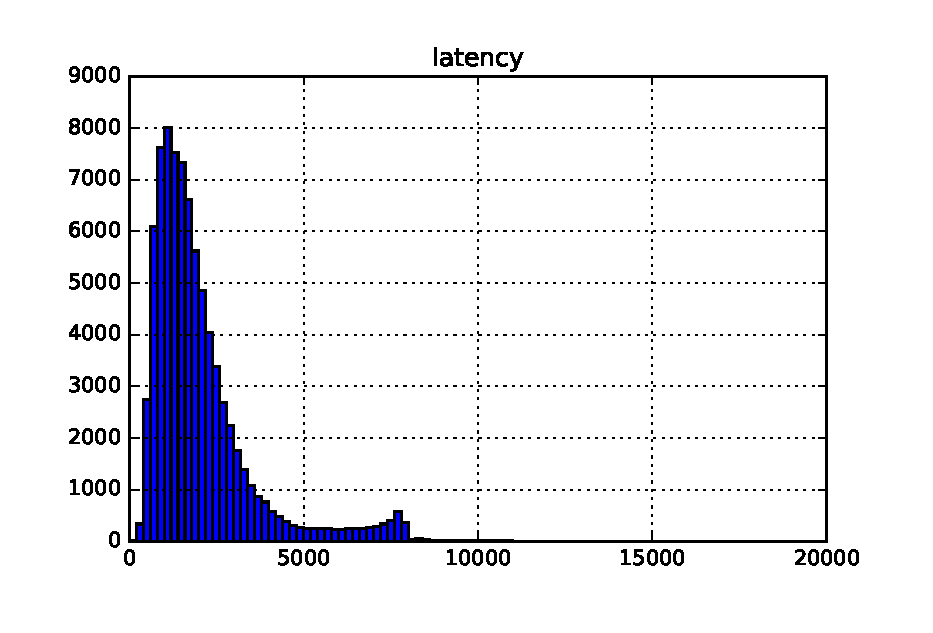
\includegraphics[width=\textwidth]{eps/storm_agg_4node_th_max_hist}

        \caption{Storm, 4-node, max   throughput }
    \end{subfigure}
    ~ 
    \begin{subfigure}[b]{0.3\textwidth}
        \includegraphics[width=\textwidth]{eps/storm_agg_8node_th_max_hist}

        \caption{Storm, 8-node, max  throughput }
        
    \end{subfigure}



    \begin{subfigure}[b]{0.3\textwidth}
        \includegraphics[width=\textwidth]{eps/spark_agg_2node_th_max_hist}

        \caption{Spark, 2-node, max  throughput }
    \end{subfigure}
    ~ 
    \begin{subfigure}[b]{0.3\textwidth}
        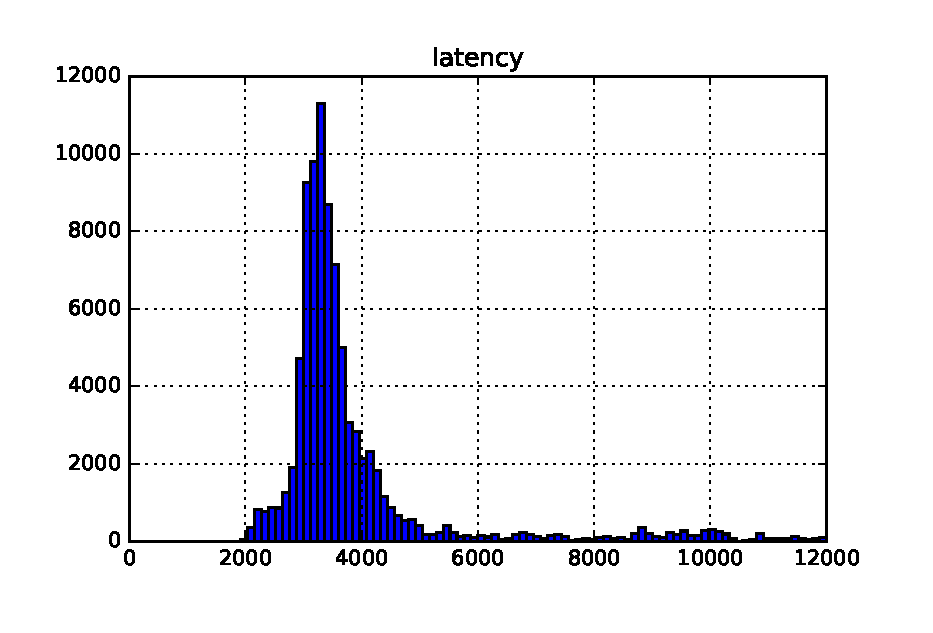
\includegraphics[width=\textwidth]{eps/spark_agg_4node_th_max_hist}

        \caption{Spark, 4-node, max  throughput }
    \end{subfigure}
    ~ 
    \begin{subfigure}[b]{0.3\textwidth}
        \includegraphics[width=\textwidth]{eps/spark_agg_8node_th_max_hist}

        \caption{Spark, 8-node, max  throughput }
        
    \end{subfigure}



    \begin{subfigure}[b]{0.3\textwidth}
        \includegraphics[width=\textwidth]{eps/flink_agg_2node_th_max_hist}

        \caption{Flink, 2-node, max  throughput }
    \end{subfigure}
    ~ 
    \begin{subfigure}[b]{0.3\textwidth}
        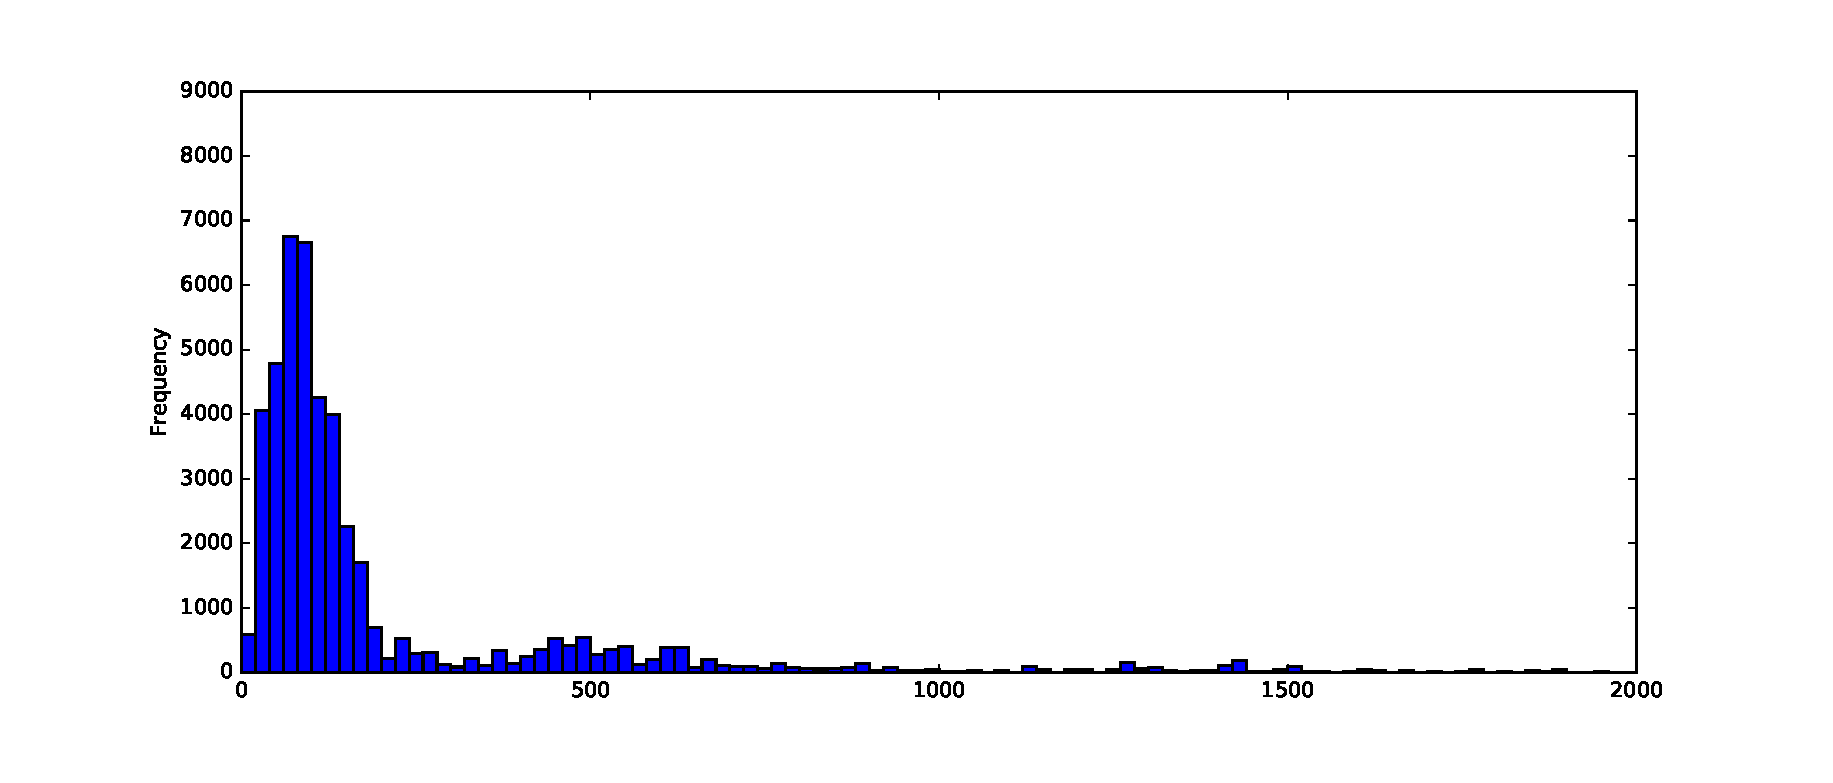
\includegraphics[width=\textwidth]{eps/flink_agg_4node_th_max_hist}

        \caption{Flink, 4-node, max  throughput }
    \end{subfigure}
    ~ 
    \begin{subfigure}[b]{0.3\textwidth}
        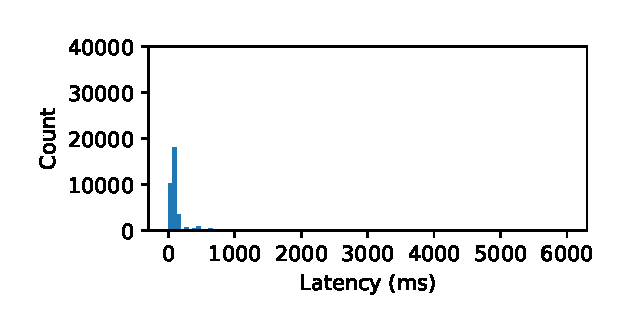
\includegraphics[width=\textwidth]{eps/flink_agg_8node_th_max_hist}

        \caption{Flink, 8-node, max  throughput }
        
    \end{subfigure}




    \begin{subfigure}[b]{0.3\textwidth}
        \includegraphics[width=\textwidth]{eps/storm_agg_2node_th_90_hist}

        \caption{Storm, 2-node, 90\%- throughput }
    \end{subfigure}
    ~ 
    \begin{subfigure}[b]{0.3\textwidth}
        \includegraphics[width=\textwidth]{eps/storm_agg_4node_th_90_hist}

        \caption{Storm, 4-node, 90\%- throughput }
    \end{subfigure}
    ~ 
    \begin{subfigure}[b]{0.3\textwidth}
        \includegraphics[width=\textwidth]{eps/storm_agg_8node_th_90_hist}

        \caption{Storm, 8-node,  90\%-throughput }
        
    \end{subfigure}



    \begin{subfigure}[b]{0.3\textwidth}
        \includegraphics[width=\textwidth]{eps/spark_agg_2node_th_90_hist}

        \caption{Spark, 2-node,  90\%-throughput }
    \end{subfigure}
    ~ 
    \begin{subfigure}[b]{0.3\textwidth}
        \includegraphics[width=\textwidth]{eps/spark_agg_4node_th_90_hist}

        \caption{Spark, 4-node,  90\%-throughput }
    \end{subfigure}
    ~ 
    \begin{subfigure}[b]{0.3\textwidth}
        \includegraphics[width=\textwidth]{eps/spark_agg_8node_th_90_hist}

        \caption{Spark, 8-node,  90\%-throughput }
        
    \end{subfigure}



    \begin{subfigure}[b]{0.3\textwidth}
        \includegraphics[width=\textwidth]{eps/flink_agg_2node_th_90_hist}

        \caption{Flink, 2-node,  90\%-throughput }
    \end{subfigure}
    ~ 
    \begin{subfigure}[b]{0.3\textwidth}
        \includegraphics[width=\textwidth]{eps/flink_agg_4node_th_90_hist}

        \caption{Flink, 4-node,  90\%-throughput }
    \end{subfigure}
    ~ 
    \begin{subfigure}[b]{0.3\textwidth}
        \includegraphics[width=\textwidth]{eps/flink_agg_8node_th_90_hist}

        \caption{Flink, 8-node,  90\%-throughput }
        
    \end{subfigure}

        \caption{Windowed aggregation latency distributions in histogram}
                \label{fig_hist_agg}
\end{figure*}

















\begin{figure*}
    \centering
    \begin{subfigure}[b]{0.3\textwidth}
        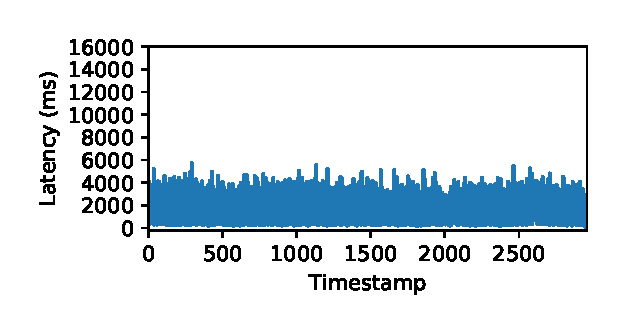
\includegraphics[width=\textwidth]{eps/storm_agg_2node_th_max_ts}

        \caption{Storm, 2-node, max   throughput }
    \end{subfigure}
    ~ 
    \begin{subfigure}[b]{0.3\textwidth}
        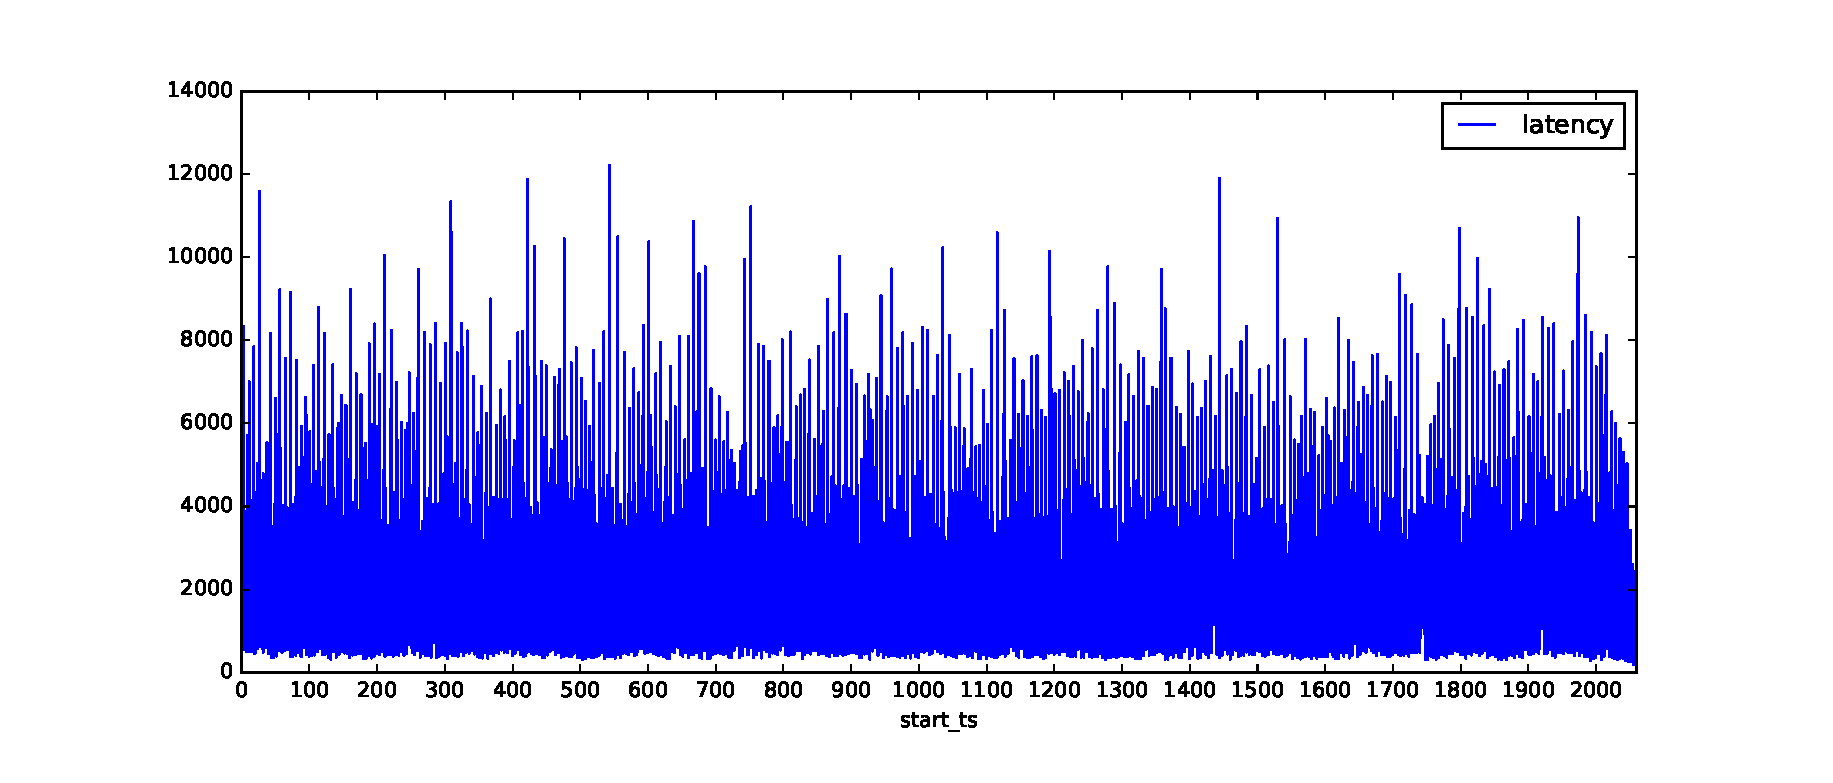
\includegraphics[width=\textwidth]{eps/storm_agg_4node_th_max_ts}

        \caption{Storm, 4-node, max   throughput }
    \end{subfigure}
    ~ 
    \begin{subfigure}[b]{0.3\textwidth}
        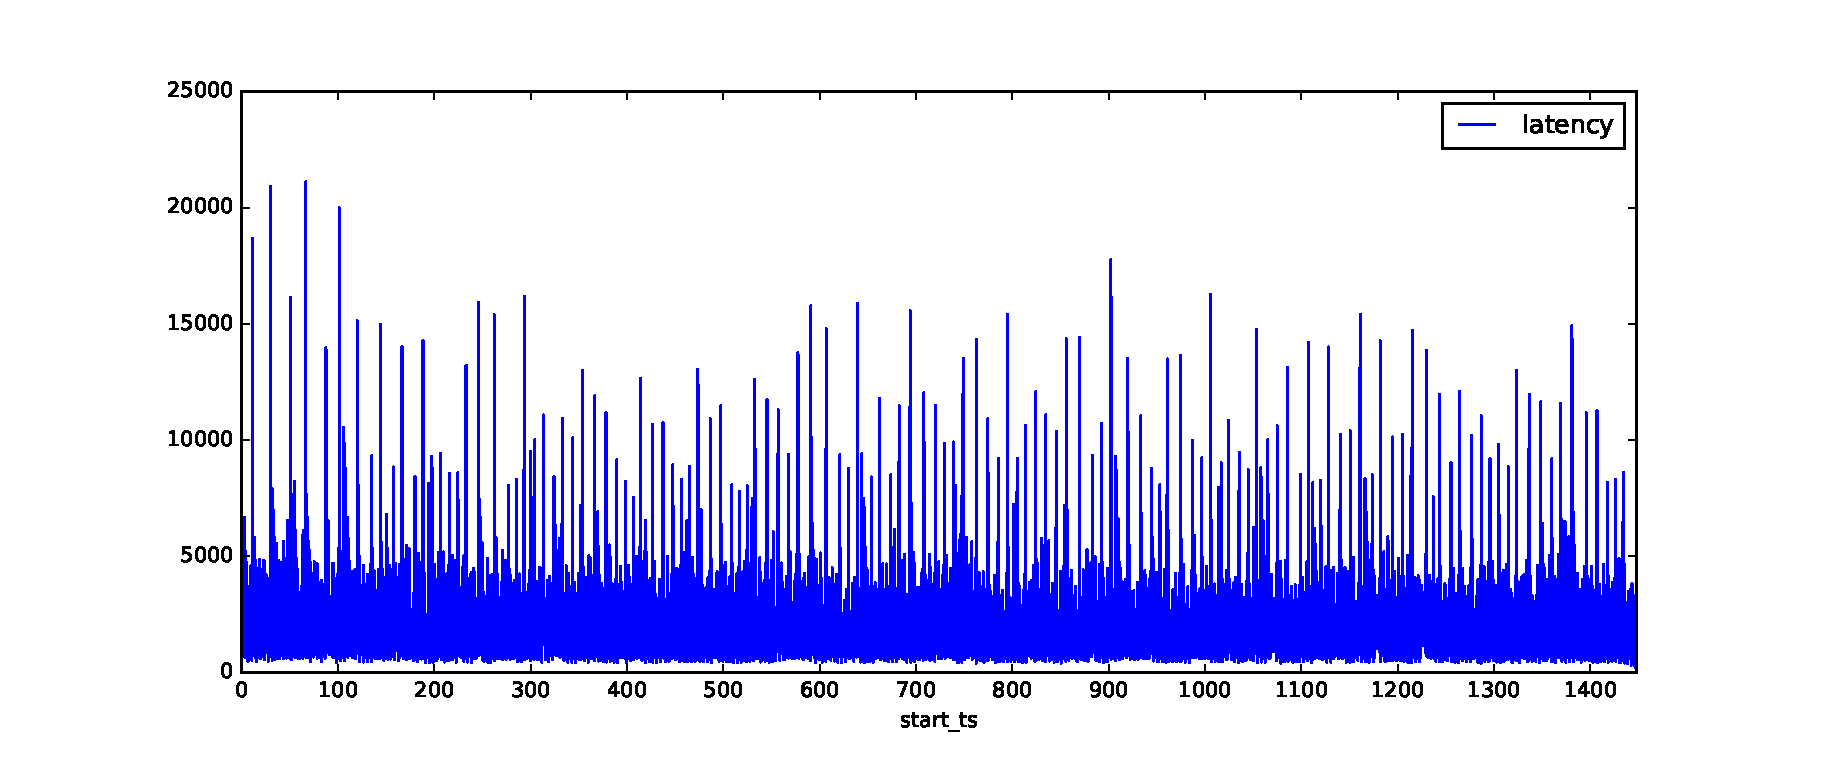
\includegraphics[width=\textwidth]{eps/storm_agg_8node_th_max_ts}

        \caption{Storm, 8-node, max   throughput }
                 \label{fig_storm_agg_8node_th_max_ts}
    \end{subfigure}



    \begin{subfigure}[b]{0.3\textwidth}
        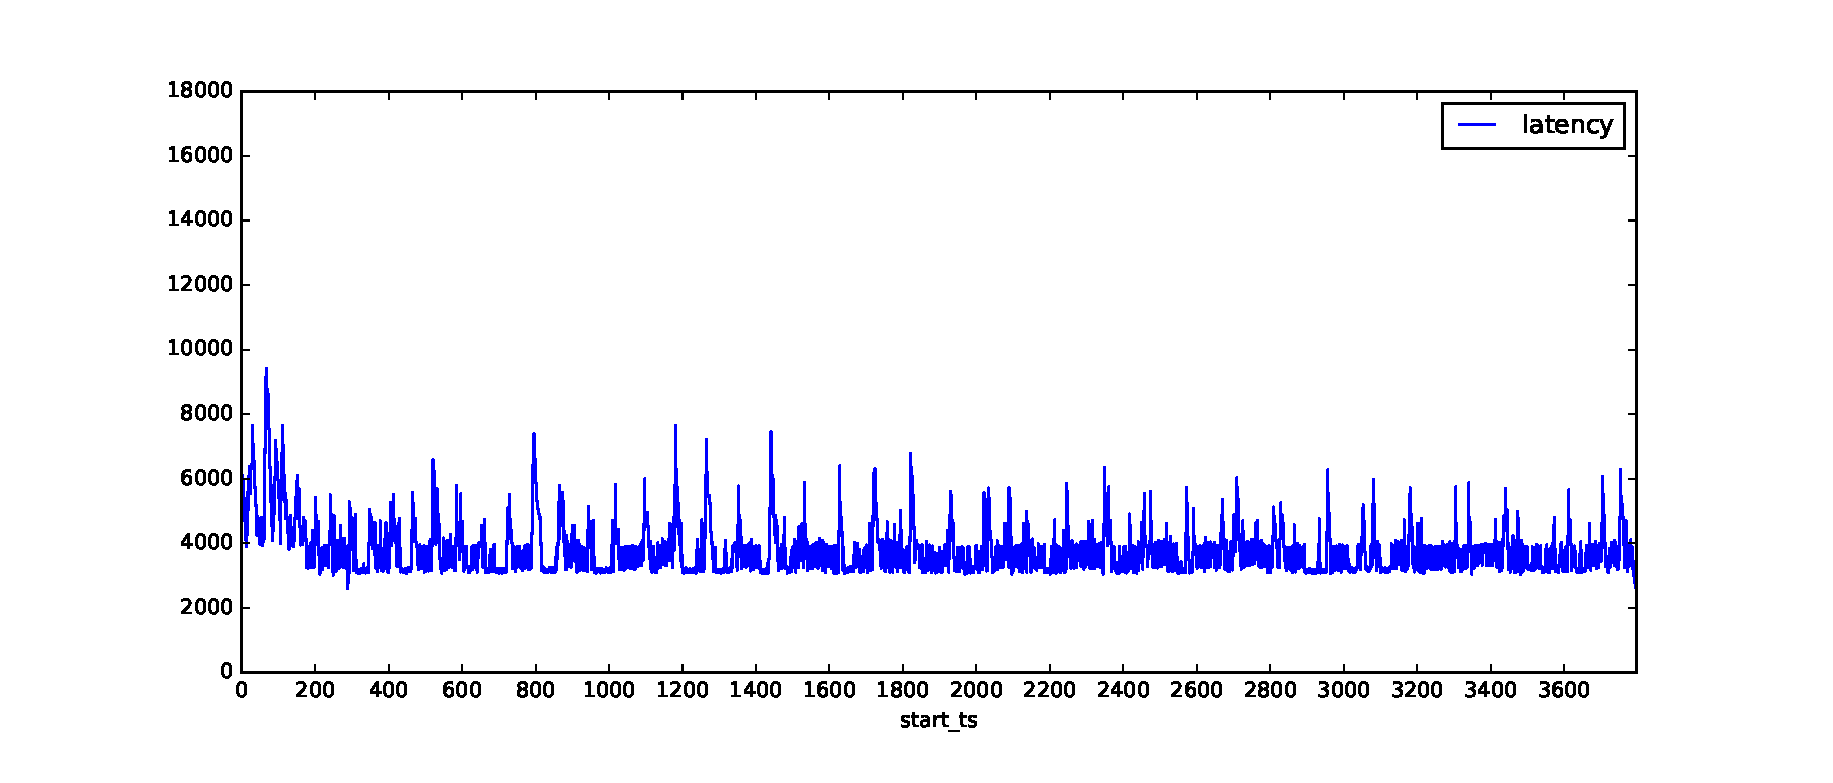
\includegraphics[width=\textwidth]{eps/spark_agg_2node_th_max_ts}

        \caption{Spark, 2-node, max   throughput }
    \end{subfigure}
    ~ 
    \begin{subfigure}[b]{0.3\textwidth}
        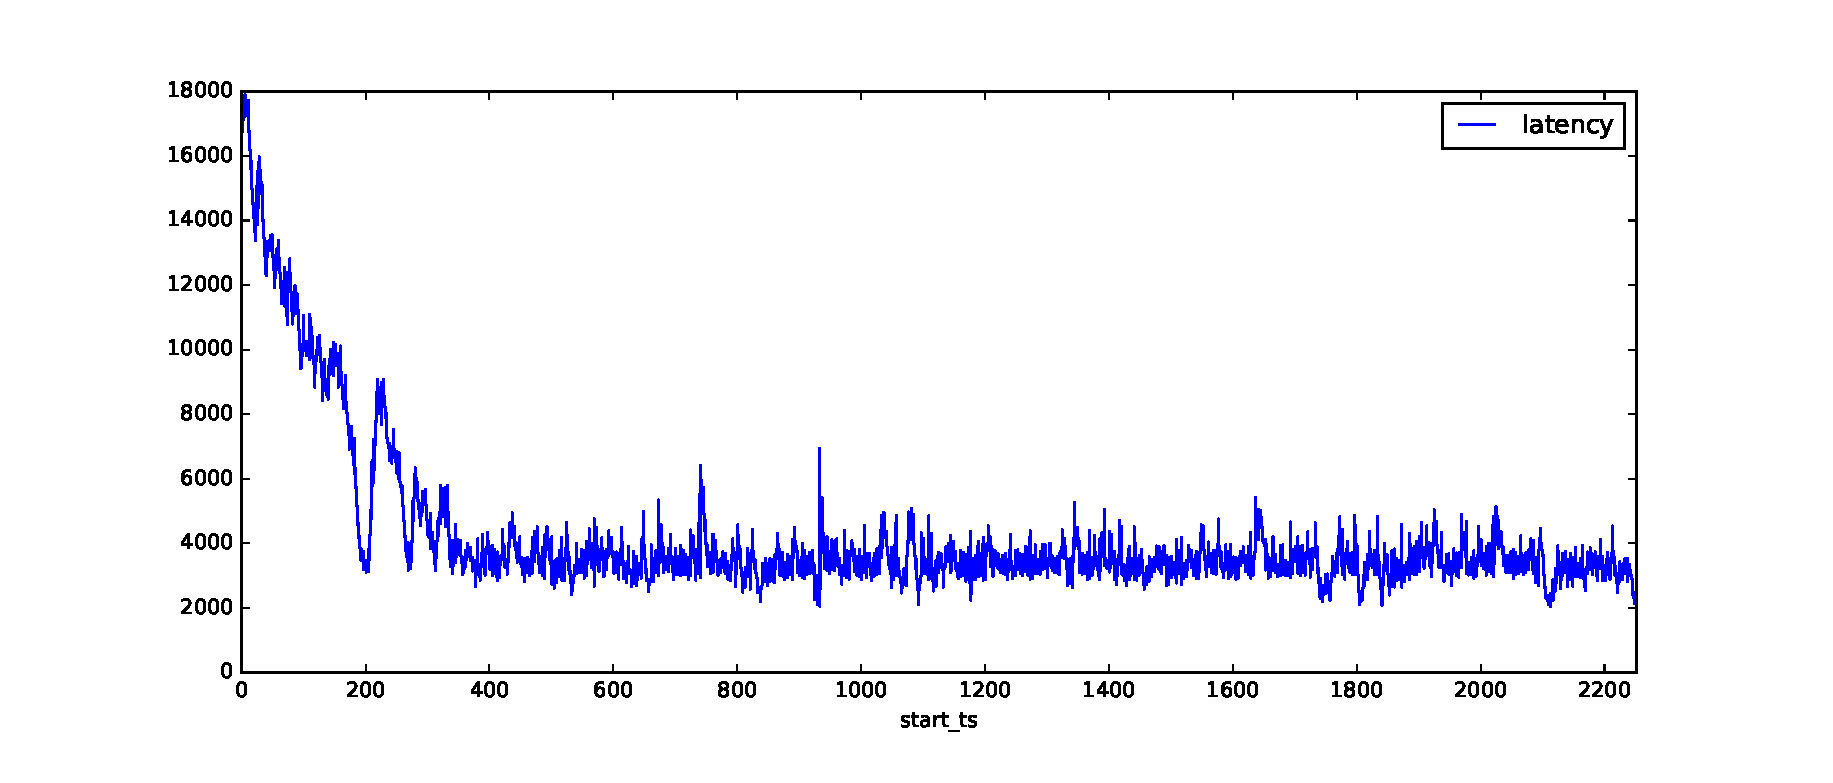
\includegraphics[width=\textwidth]{eps/spark_agg_4node_th_max_ts}

        \caption{Spark, 4-node, max   throughput }
    \end{subfigure}
    ~ 
    \begin{subfigure}[b]{0.3\textwidth}
        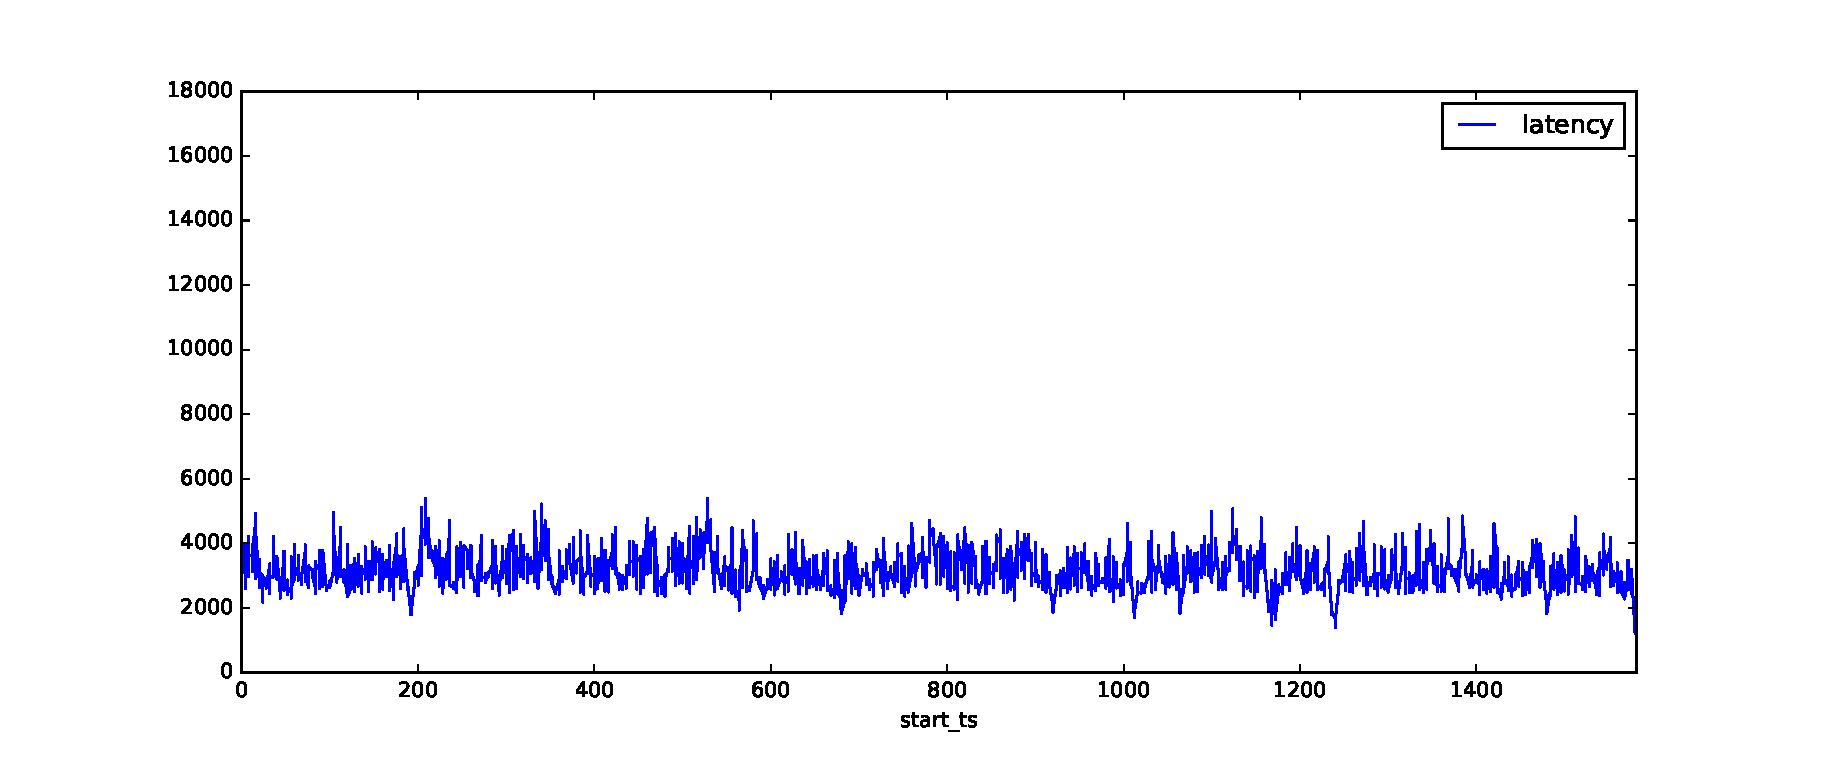
\includegraphics[width=\textwidth]{eps/spark_agg_8node_th_max_ts}

        \caption{Spark, 8-node, max   throughput }
         \label{fig_spark_agg_8node_th_max_ts}
    \end{subfigure}



    \begin{subfigure}[b]{0.3\textwidth}
        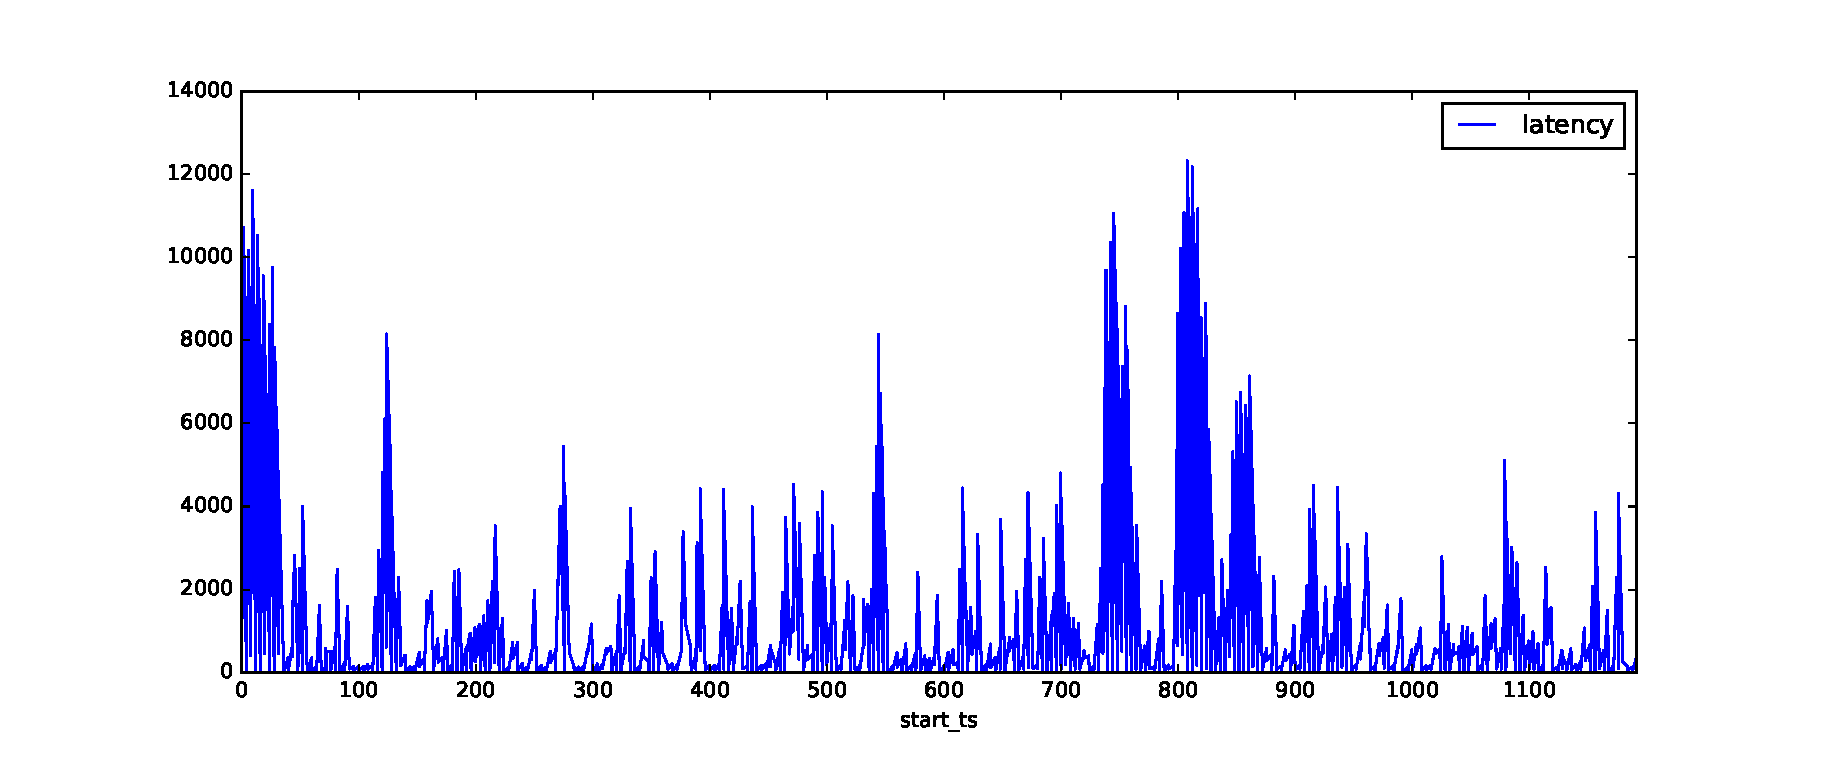
\includegraphics[width=\textwidth]{eps/flink_agg_2node_th_max_ts}

        \caption{Flink, 2-node, max   throughput }
                \label{flink_agg_2node_th_max_ts}

    \end{subfigure}
    ~ 
    \begin{subfigure}[b]{0.3\textwidth}
        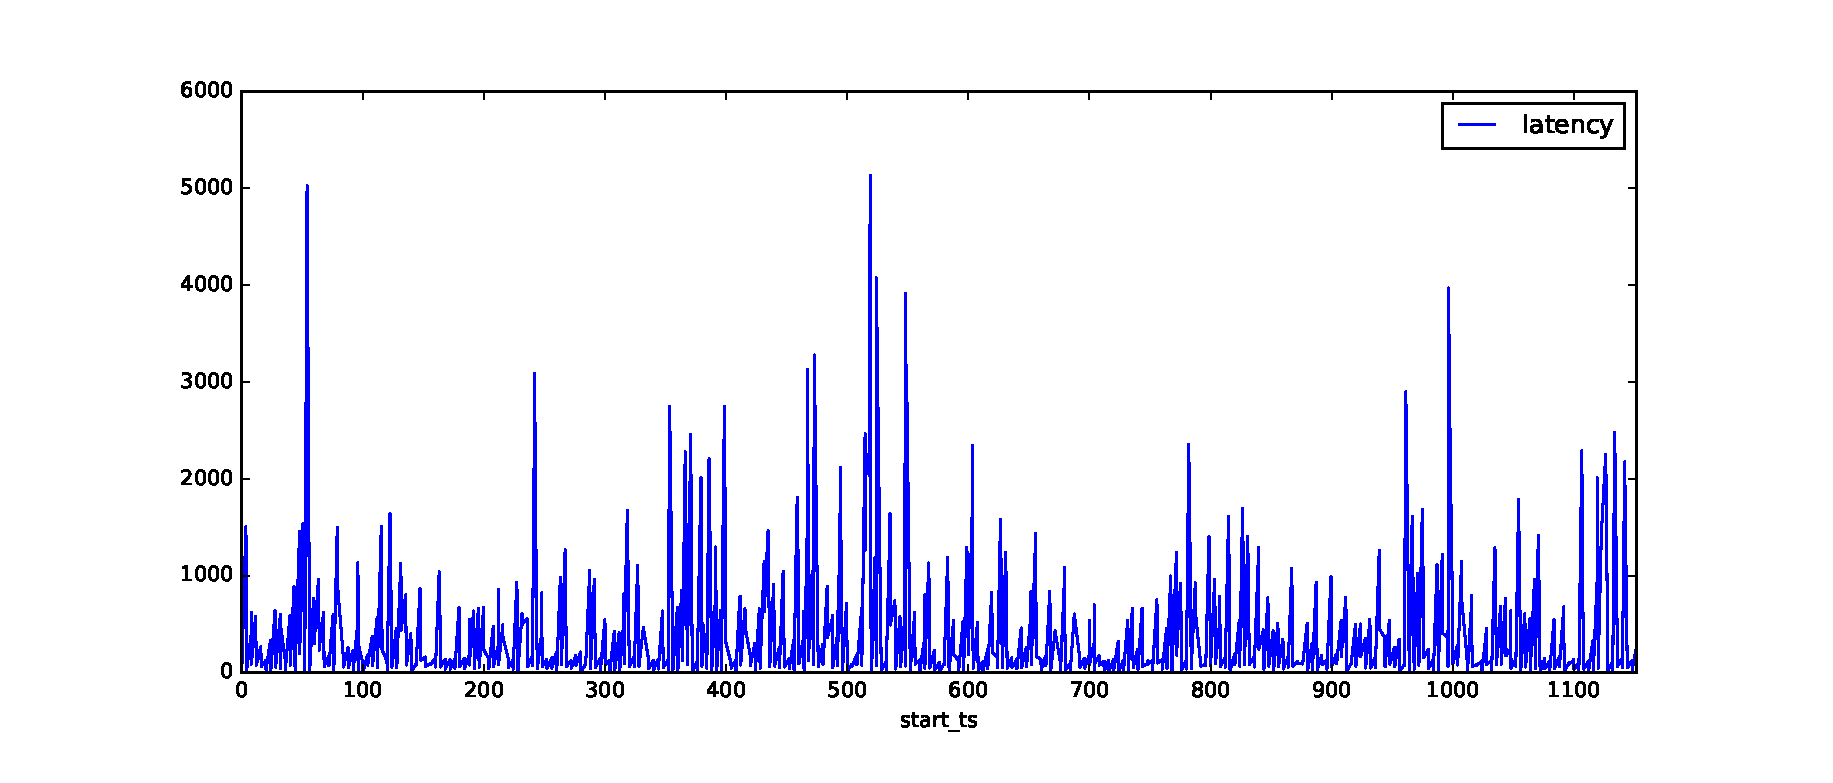
\includegraphics[width=\textwidth]{eps/flink_agg_4node_th_max_ts}

        \caption{Flink, 4-node, max   throughput }
    \end{subfigure}
    ~ 
    \begin{subfigure}[b]{0.3\textwidth}
        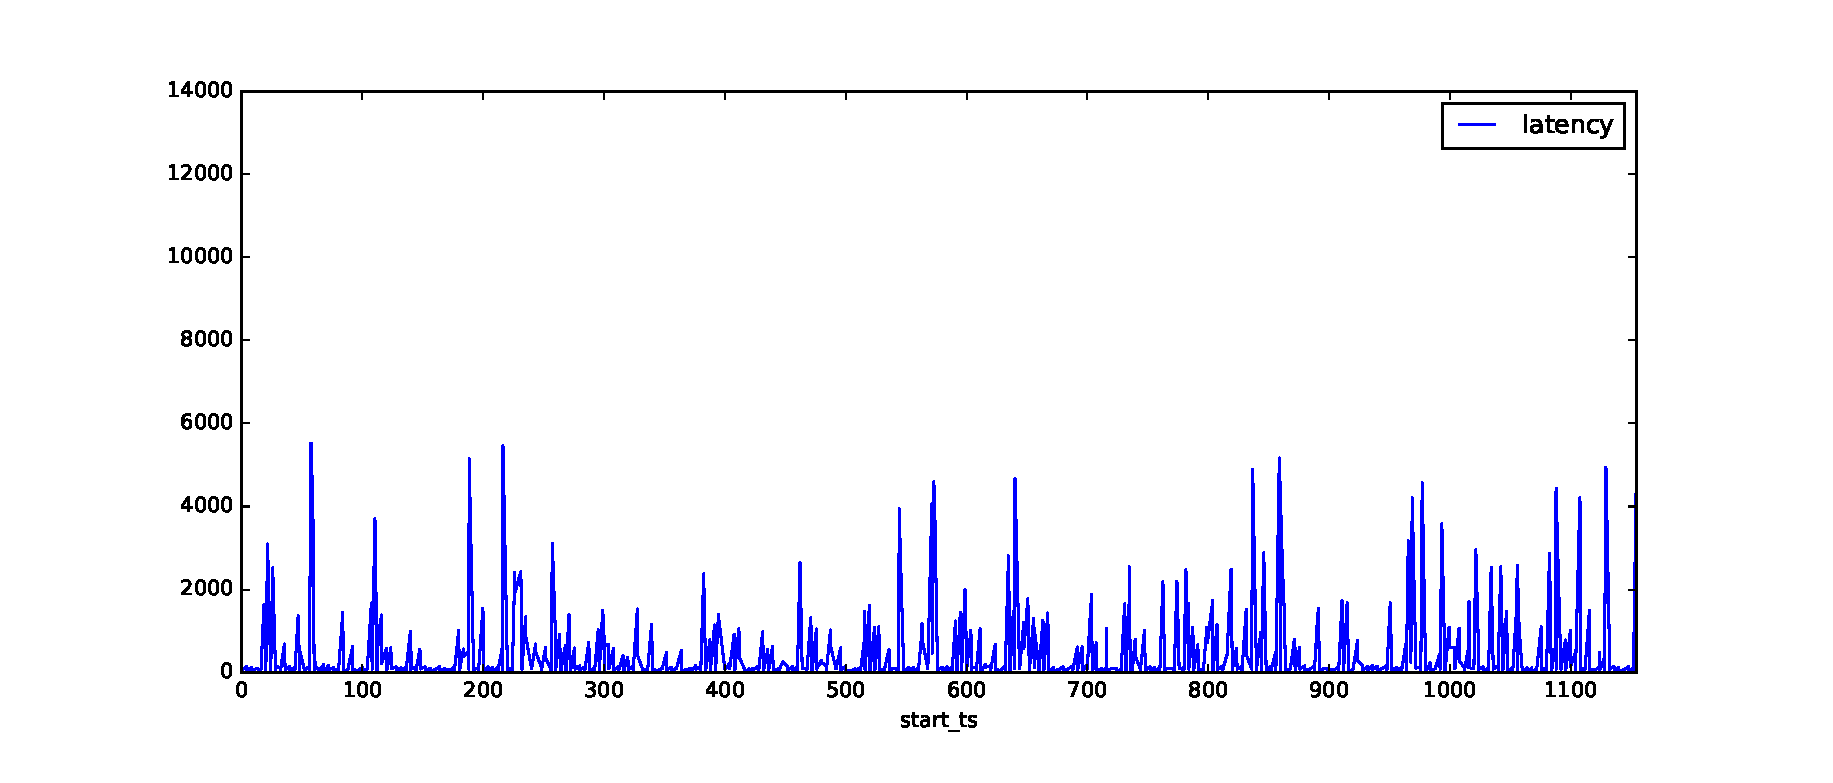
\includegraphics[width=\textwidth]{eps/flink_agg_8node_th_max_ts}

        \caption{Flink, 8-node, max   throughput }
        
    \end{subfigure}




    \begin{subfigure}[b]{0.3\textwidth}
        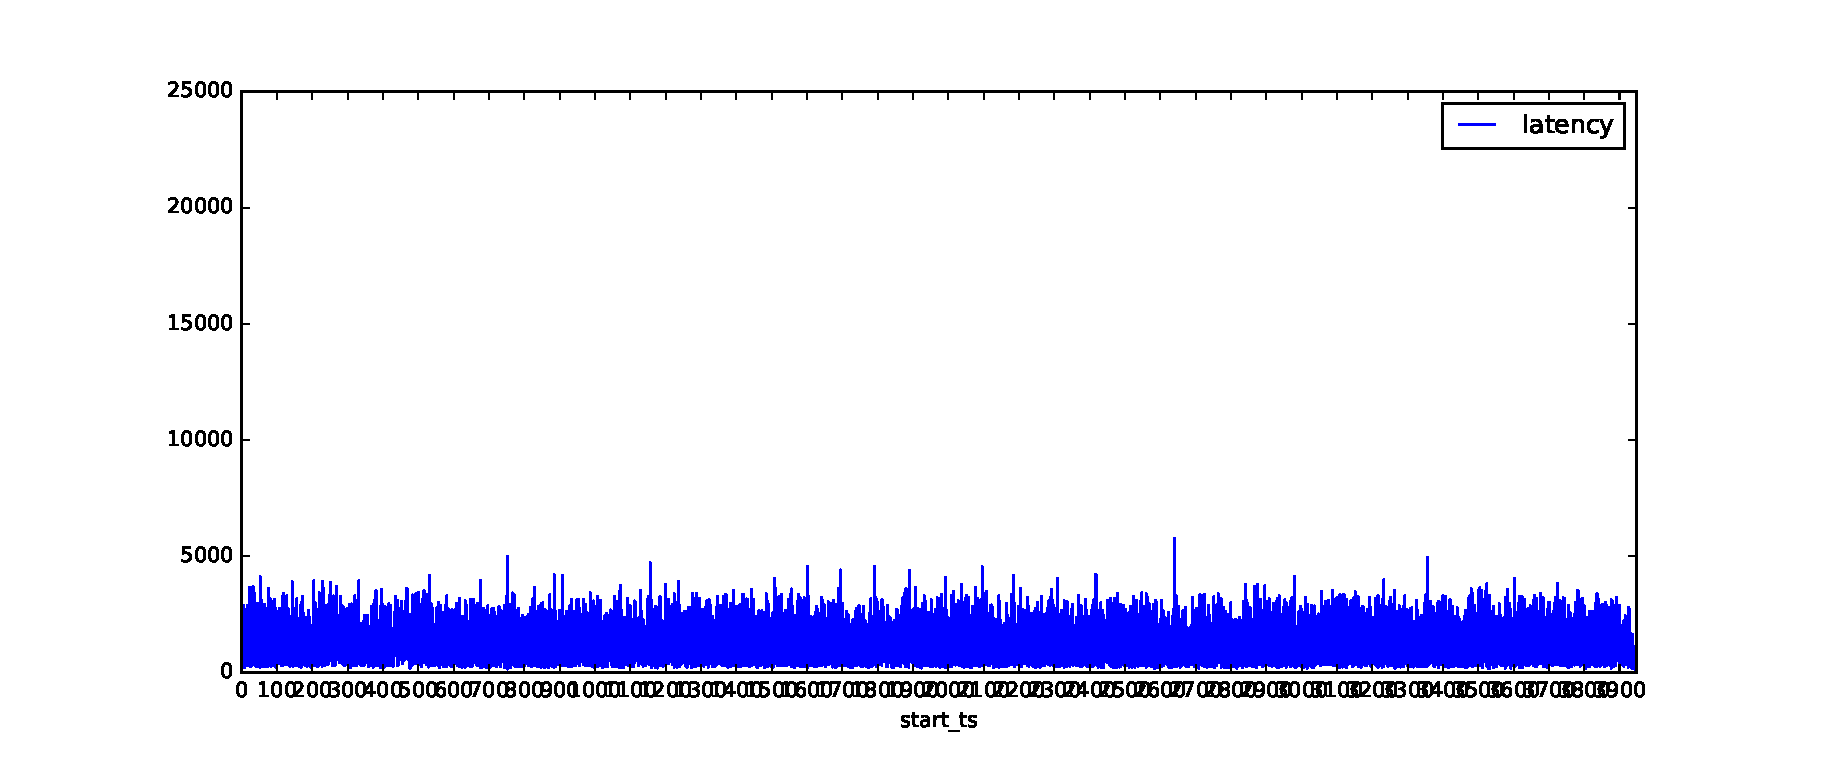
\includegraphics[width=\textwidth]{eps/storm_agg_2node_th_90_ts}

        \caption{Storm, 2-node,  90\%- throughput }
    \end{subfigure}
    ~ 
    \begin{subfigure}[b]{0.3\textwidth}
        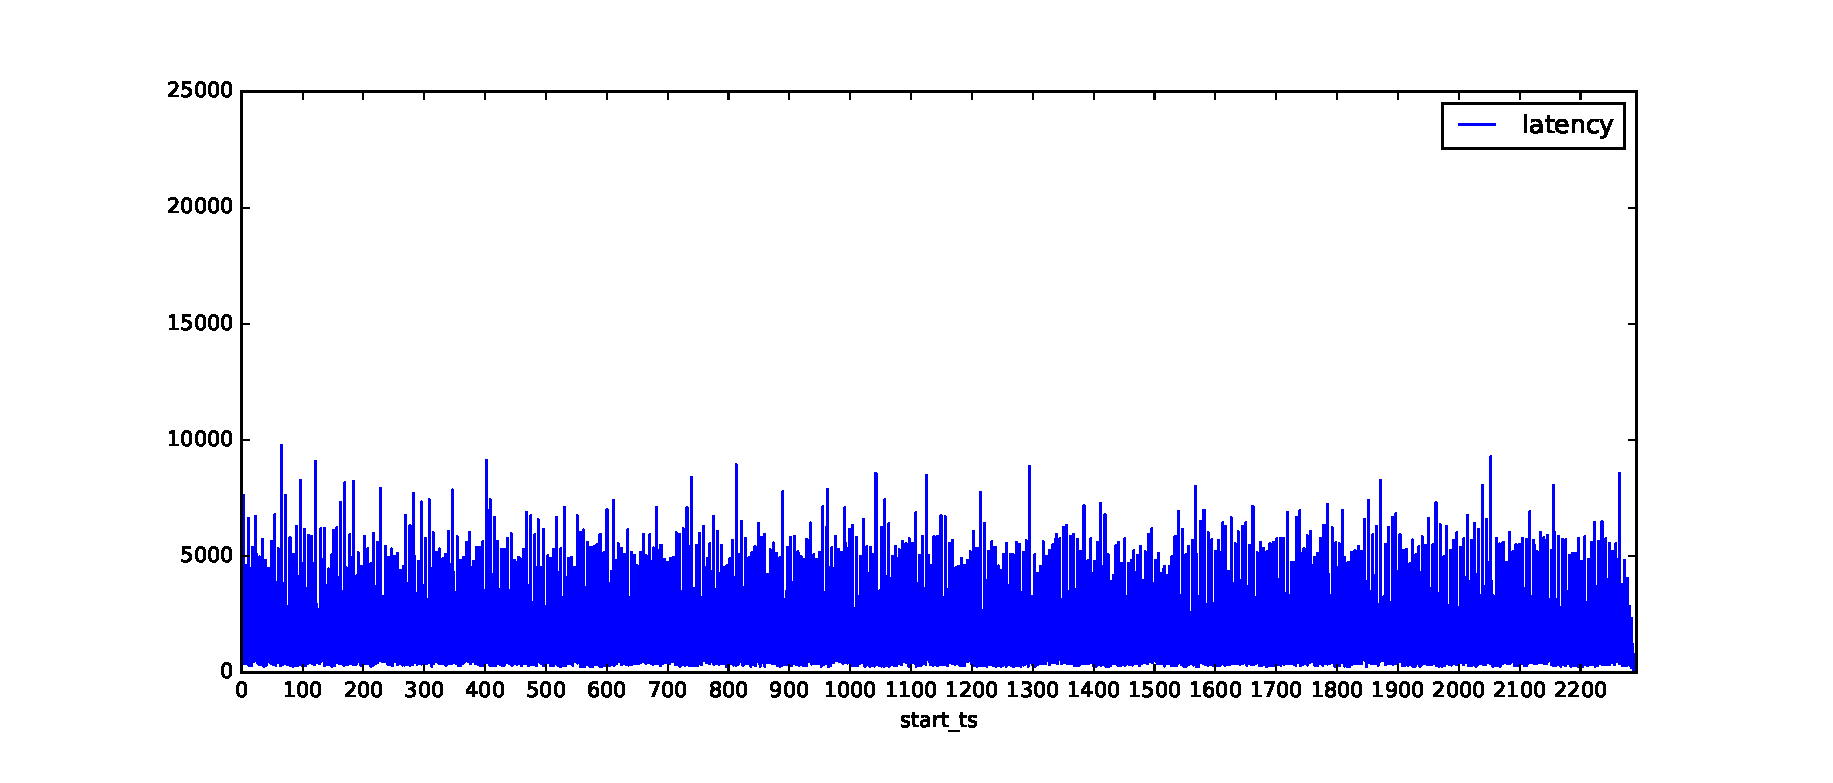
\includegraphics[width=\textwidth]{eps/storm_agg_4node_th_90_ts}

        \caption{Storm, 4-node,  90\%- throughput }
    \end{subfigure}
    ~ 
    \begin{subfigure}[b]{0.3\textwidth}
        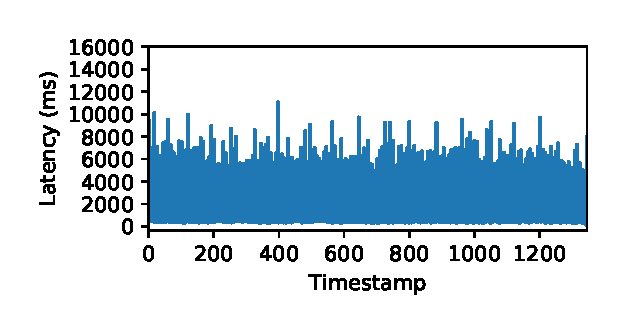
\includegraphics[width=\textwidth]{eps/storm_agg_8node_th_90_ts}

        \caption{Storm, 8-node,  90\%- throughput }
                \label{fig_storm_agg_8node_th_90_ts}
    \end{subfigure}



    \begin{subfigure}[b]{0.3\textwidth}
        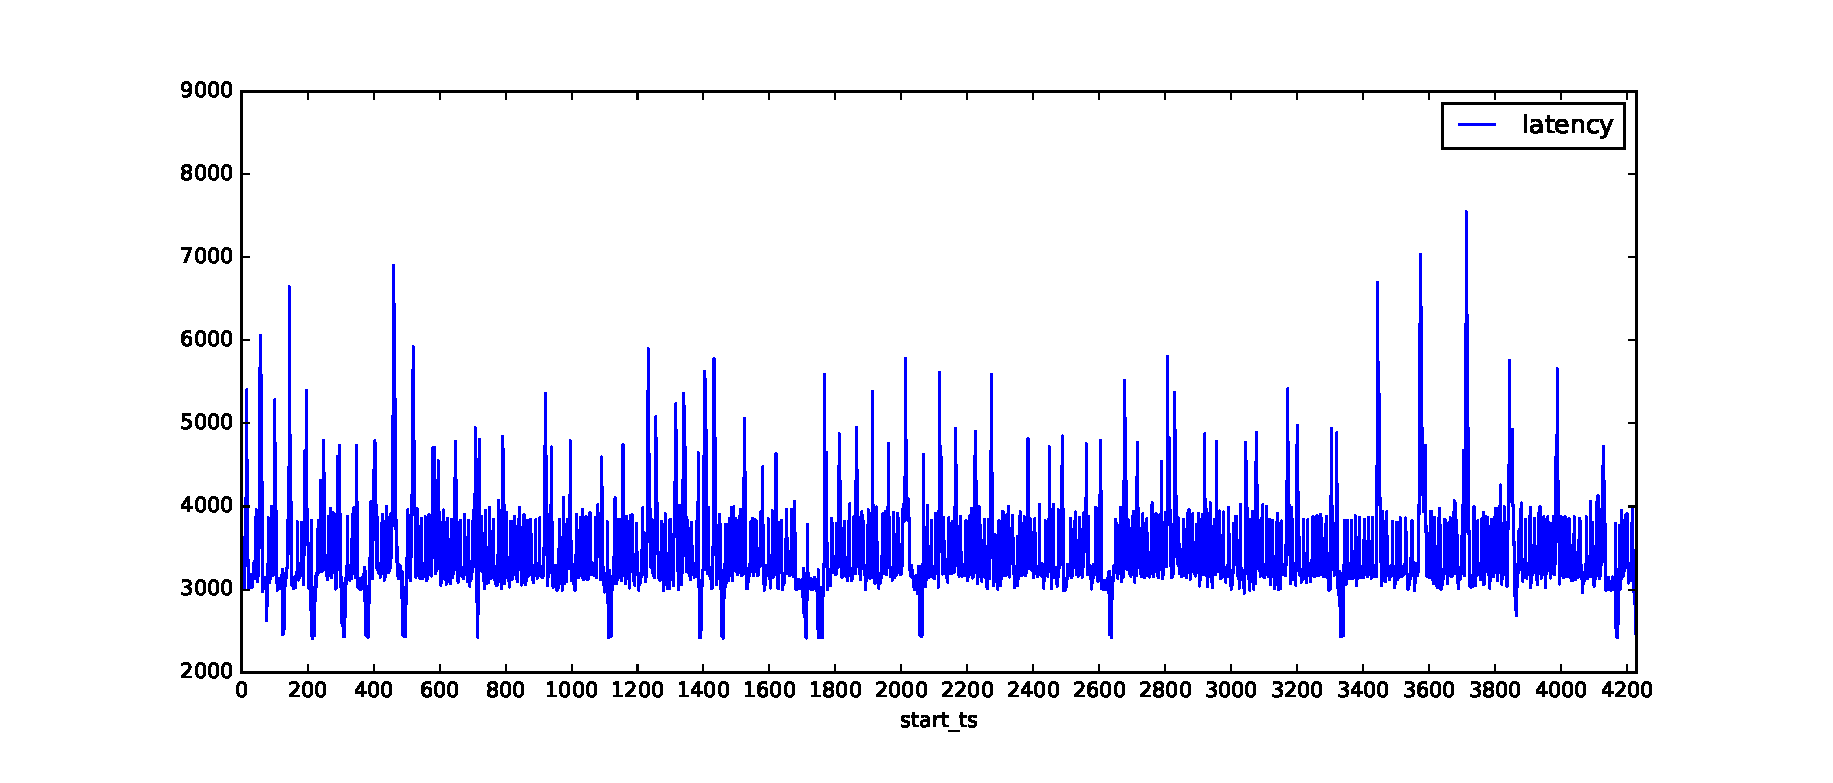
\includegraphics[width=\textwidth]{eps/spark_agg_2node_th_90_ts}

        \caption{Spark, 2-node,  90\%- throughput }
    \end{subfigure}
    ~ 
    \begin{subfigure}[b]{0.3\textwidth}
        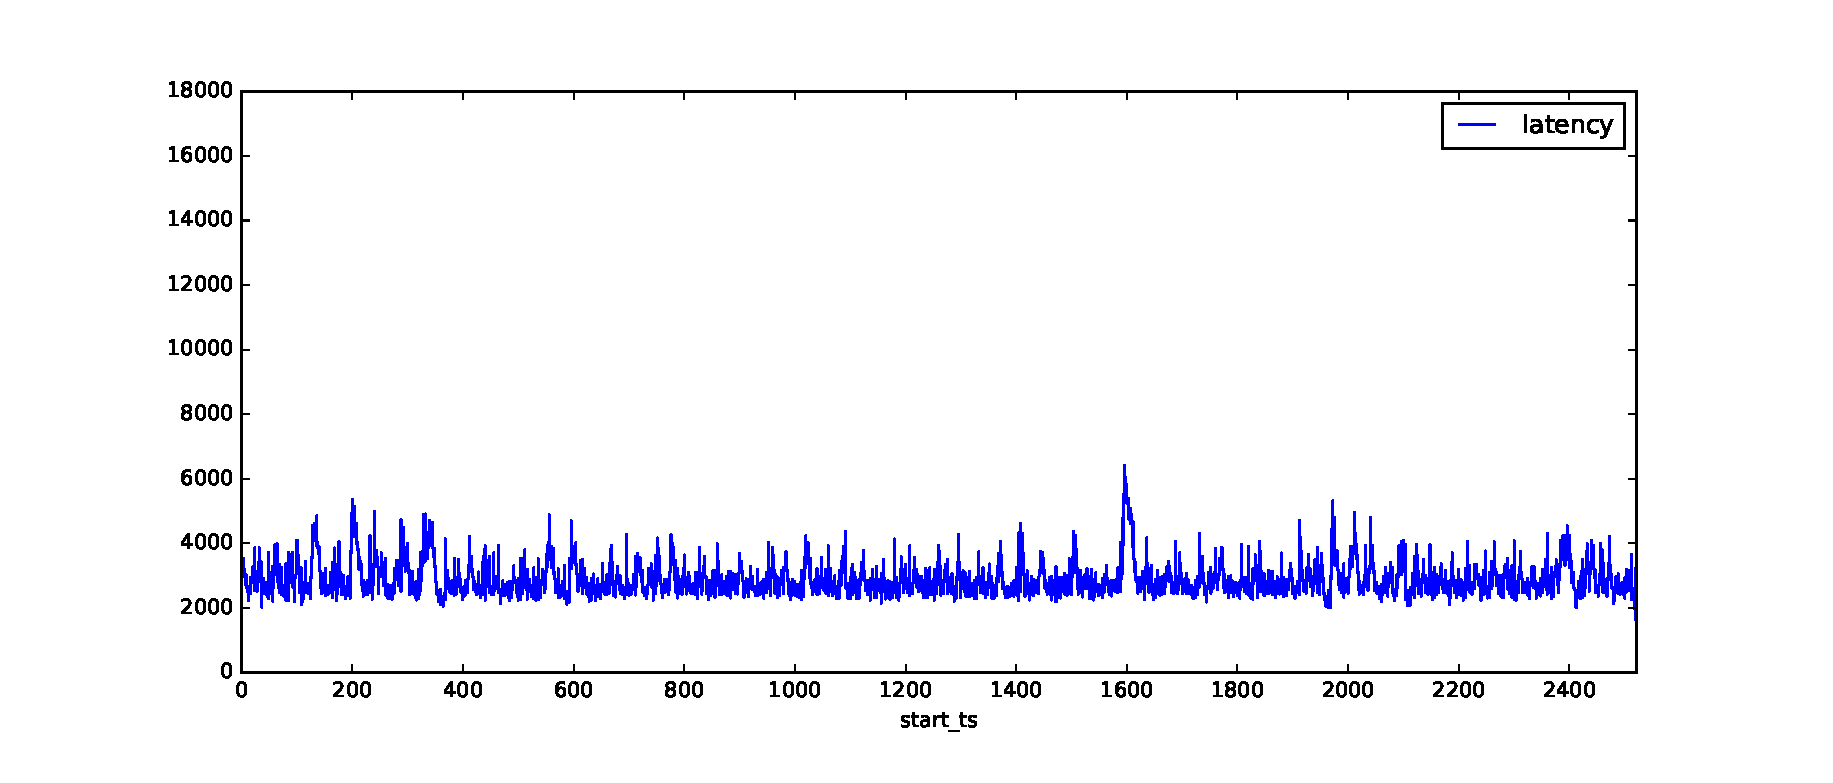
\includegraphics[width=\textwidth]{eps/spark_agg_4node_th_90_ts}

        \caption{Spark, 4-node,  90\%- throughput }
    \end{subfigure}
    ~ 
    \begin{subfigure}[b]{0.3\textwidth}
        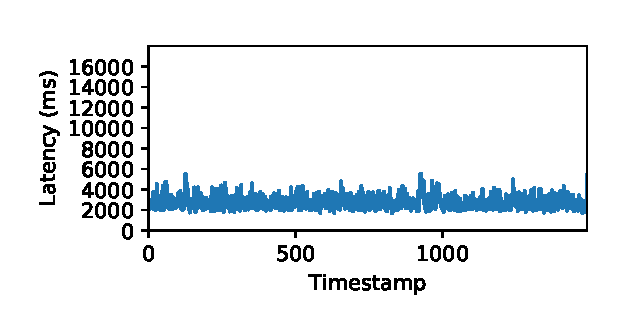
\includegraphics[width=\textwidth]{eps/spark_agg_8node_th_90_ts}

        \caption{Spark, 8-node,  90\%- throughput }
        
    \end{subfigure}



    \begin{subfigure}[b]{0.3\textwidth}
        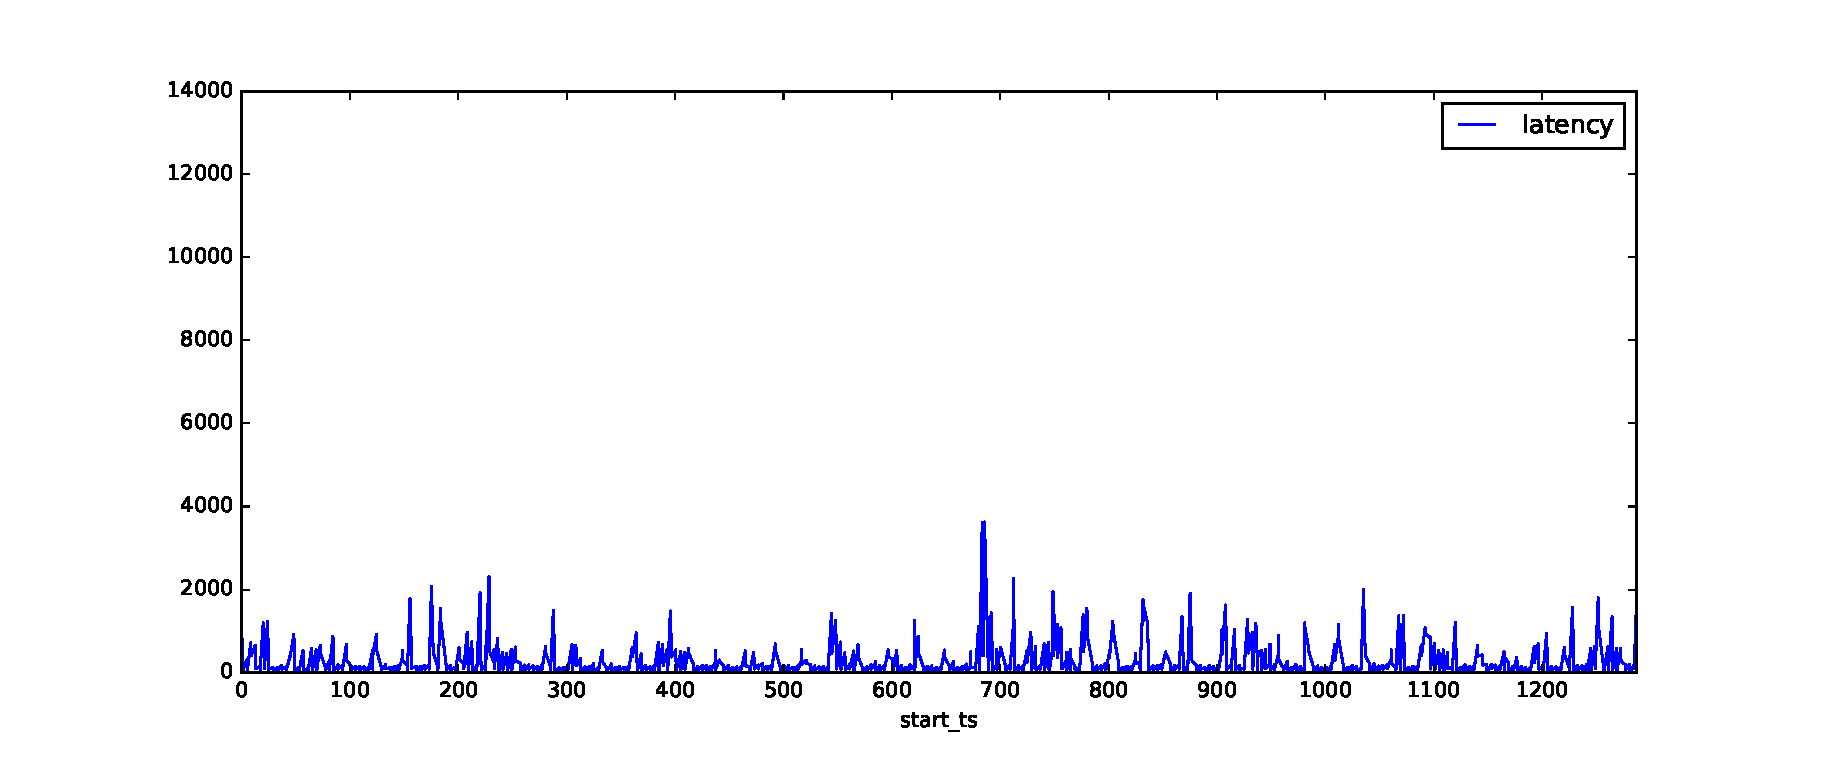
\includegraphics[width=\textwidth]{eps/flink_agg_2node_th_90_ts}

        \caption{Flink, 2-node,  90\%- throughput }
        \label{fig_flink_agg_2node_th_90_ts}
    \end{subfigure}
    ~ 
    \begin{subfigure}[b]{0.3\textwidth}
        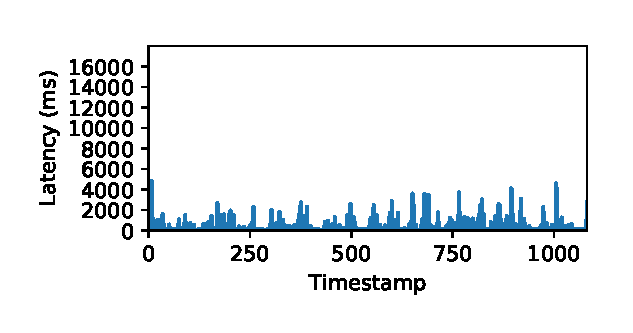
\includegraphics[width=\textwidth]{eps/flink_agg_4node_th_90_ts}

        \caption{Flink, 4-node,  90\%- throughput }
    \end{subfigure}
    ~ 
    \begin{subfigure}[b]{0.3\textwidth}
        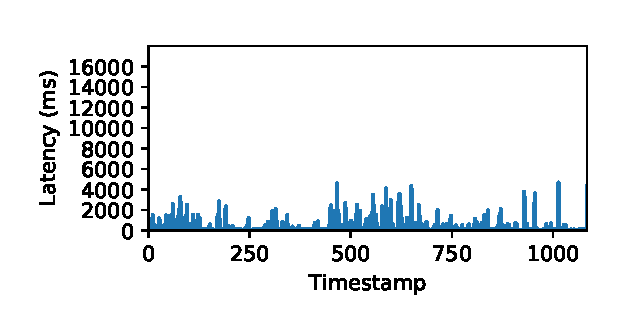
\includegraphics[width=\textwidth]{eps/flink_agg_8node_th_90_ts}

        \caption{Flink, 8-node, 90\% throughput }
        
    \end{subfigure}

        \caption{Windowed aggregation latency distributions in time series}
                \label{fig_ts_agg}
\end{figure*}









Figures \ref{fig_hist_agg} and \ref{fig_ts_agg} show the windowed aggregation latency distributions as  histogram and  time-series,  respectively. 
In all cases we can see that the fluctuations are lowered when decreasing the throughput by 10\%.  While in Storm and in Flink it is hard to detect the lower bounds of latency as they are close to zero, in Spark the upper and lower boundaries are more stable and clearly noticeable. The reason is that a Spark job's characteristics are  highly dependent on the batch size and this determines the clear upper and lower boundaries for the latency. The lower the batch size, the lower the latency and throughput. To have a stable and efficient configuration in Spark, the mini-batch processing time should be less than the batch interval.  We determine the most fluctuating system to be Flink in  2-node setup and Storm in 8-node setup  as shown in Figures \ref{flink_agg_2node_th_max_ts} and \ref{fig_storm_agg_8node_th_max_ts}. Those fluctuations show the behaviour of backpressure. For the same experiment with 90\% of the maximum throughput, we notice that the fluctuations are significantly reduced as shown in  Figures \ref{fig_flink_agg_2node_th_90_ts} and \ref{fig_storm_agg_8node_th_90_ts}.
As we discussed above, 4- and 8-node experiments in Flink are network bound; therefore, these experiments do not fully utilize the Flink nodes and thus have a lower variance in latency. 



Figure \ref{fig_cpu_network_metrics} shows the resource usages of the SUTs. The upper figure shows the CPU load during the experiment. The CPU load is the number of kernel level threads  that are runnable and queued while waiting for CPU resources, averaged over one minute. The next figure shows the network usage of the SUTs.  Because the overall result is similar, we show the of systems' resource utilization graphs  with windowed aggregation case in 4-node cluster.  Because Flink's performance is bounded by network, we can see that CPU utilization is minimal among others. Storm, on the other hand, uses approximately 50\% more CPU clock cycles than Spark. This results in having competitively higher throughout than Spark. One reason behind  Spark's efficient usage of CPU is that Spark automizes most of the work, handles resource usages transparent to user, and does a lot of optimizations internally. For example, Spark handles incremental state management, optimizations with code generation and dynamic memory management efficiently and transparent to user. 



    \begin{table}
        \begin{tabular}{lllll}\toprule
            &\textbf{2-node}  & \textbf{4-node} & \textbf{8-node}\\\midrule
            Spark & 365K & 632K & 947K  \\
            Flink & 851K & 1128K & 1190K \\
        \end{tabular}
        \caption{Sustainable throughput for windowed joins}
                 \label{tab_th_join}
    \end{table} 


\setlength{\tabcolsep}{0.1em} % for the horizontal padding
{\renewcommand{\arraystretch}{1.0}% for the vertical padding
    \begin{table*}
        \resizebox{\textwidth}{!} {\begin{tabular}{lllll}\toprule
            &\textbf{2-node}  & \textbf{4-node} & \textbf{8-node}\\\midrule
            Spark & 7724, 1376, 21600, (11297, 12409, 14718) & 6730, 2139, 23647, (10279, 11788, 15410) & 6263, 1841, 19993, (9465, 10469, 13242) \\
            Spark(90\%) & 7195, 2157, 17981, (10316, 11178, 12702) & 5834, 1861, 13956, (8741, 9525, 10729) & 5788, 1721, 14197, (8678, 9454, 10625)\\
            Flink & 4367, 17, 18230, (7601, 8570, 10554) & 3671, 19, 13872, (6756, 7531, 8664) & 3275, 22, 14934, (6241, 7045, 8436) \\
            Flink(90\%) & 3866, 19, 13027, (6786, 7569, 8759) & 3243, 16, 12702, (6130, 6901, 8011)  & 3240, 16, 14978, (6199, 6995, 8304) \\
        \end{tabular}}
        \caption{Latency statistics, avg, min, max and quantiles (25, 50, 75) in milliseconds for windowed joins.}
                 \label{tab_lat_join}
    \end{table*} 


\begin{figure*}
   \centering

   \begin{subfigure}[b]{0.3\textwidth}
       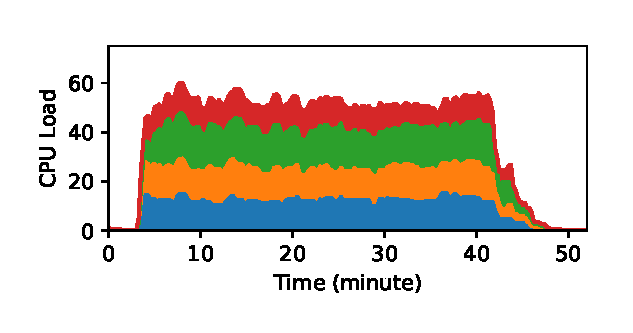
\includegraphics[width=\textwidth]{eps/storm_load_one}
        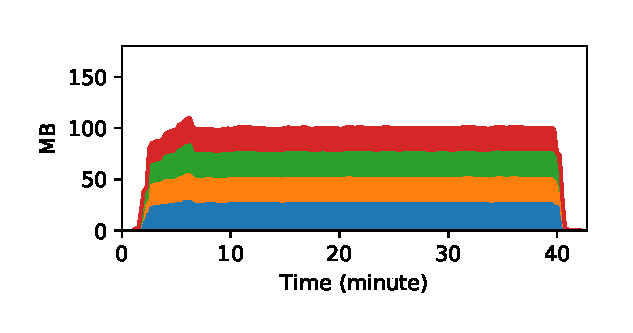
\includegraphics[width=\textwidth]{eps/storm_bytes_in}

       \caption{CPU and network usage of Storm }
   \end{subfigure}
      ~ 
   \begin{subfigure}[b]{0.3\textwidth}
       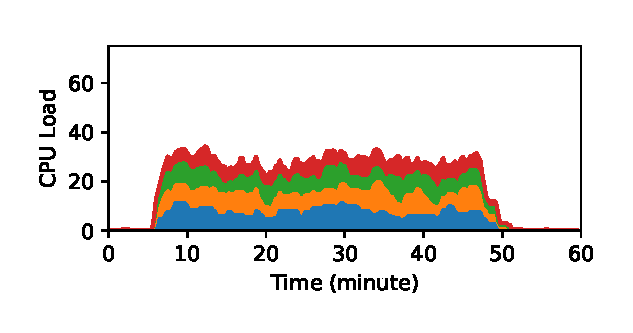
\includegraphics[width=\textwidth]{eps/spark_load_one}
        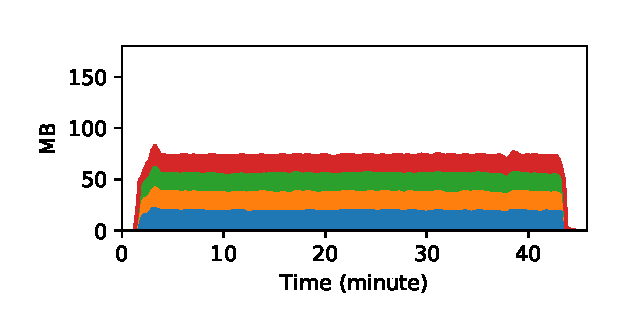
\includegraphics[width=\textwidth]{eps/spark_bytes_in}

       \caption{CPU and network usage of Spark }
   \end{subfigure}
   ~ 
   \begin{subfigure}[b]{0.3\textwidth}
       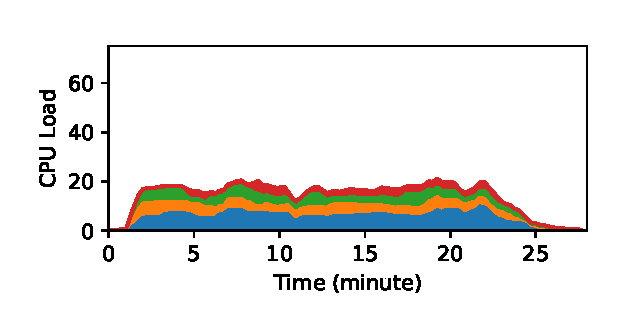
\includegraphics[width=\textwidth]{eps/flink_load_one}
        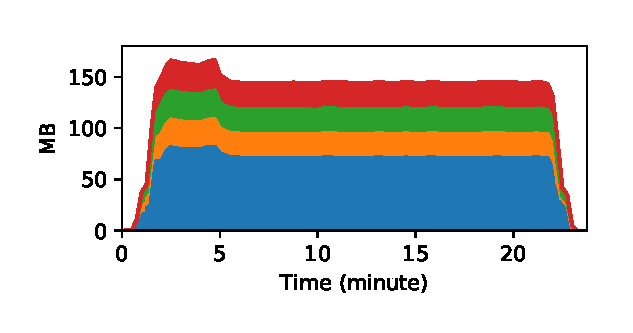
\includegraphics[width=\textwidth]{eps/flink_bytes_in}

       \caption{CPU and network usage of Flink }
   \end{subfigure}

        \caption{CPU and Network usage of systems in a 4-node cluster. Colors indicate nodes in a cluster}
        \label{fig_cpu_network_metrics}
\end{figure*}





\subsection{Windowed Joins}
In the second use-case, we use partitioned windowed joins in Spark and Flink.
  Storm provides a windowing capability but there is no built-in windowed join operator. Initially, we tried Storm's Trident abstrac\-tion, which has built-in windowed join features. However, Trident computed incorrect results as we increased the batch size. Moreover, there is a lack of support for Trident in the Storm community. As an alternative, we implemented a simple version of a windowed join in Storm. However, comparing it with Spark and Flink, which have advanced memory and state management features, leads to unfair comparisons. We implemented a na\"ive join in Storm and examined the maximum sustainable throughput to be 140K events per second and measured an average latency of 2349 milliseconds  on a 2-node cluster. However, we faced memory issues and topology stalls on larger clusters. 
%Moreover, this  would be highly implementation dependent. 
As a result, we focus on Flink and Spark in our windowed join benchmarks.

Throughout the experiments, we found important points that need to be taken into consideration while performing windowed joins over streams. First, depending on the selectivity of the input streams to the join operator, vast amount of results can be produced which can limit the speed of the engine to the disk I/O. We are assuming that the result sink is a file system. Second, the vast amount of results of a join operator can cause the network to be a bottleneck. This can happen if we output the results to shared file system. If the result size is large, then the network becomes a bottleneck. To address this issue, we decreased the selectivity of the input streams.  In general, the experimental results for windowed joins are similar to the experiments with windowed aggregations. 

Table \ref{tab_th_join} shows the maximum throughput that the systems under test can sustain.  Flink's throughput for 8-node configuration is bounded by network bandwidth. This is 1256K in windowed aggregations. The reason for the difference is that there is more network traffic as the result size is larger in windowed joins than in windowed aggregations. Tab\-le \ref{tab_lat_join} shows the latency statistics for windowed joins. We can see that  
in all cases Flink outperforms Spark in all parameters. To ensure the stability of the system, the run time of each mini-batch should be less than batch size in Spark. Otherwise, the queued mini-batch jobs will increase over time and the system will not be able to sustain the throughput. However, we see from Table \ref{tab_th_join} that the latency values are higher than mini-batch duration (4 sec). The reason is that we are measuring the event time latency.Therefore, if the latency is higher than mini-batch duration, then the tuples wait in the DQS.
















































\begin{figure*}
    \centering
   \begin{subfigure}[b]{0.3\textwidth}
       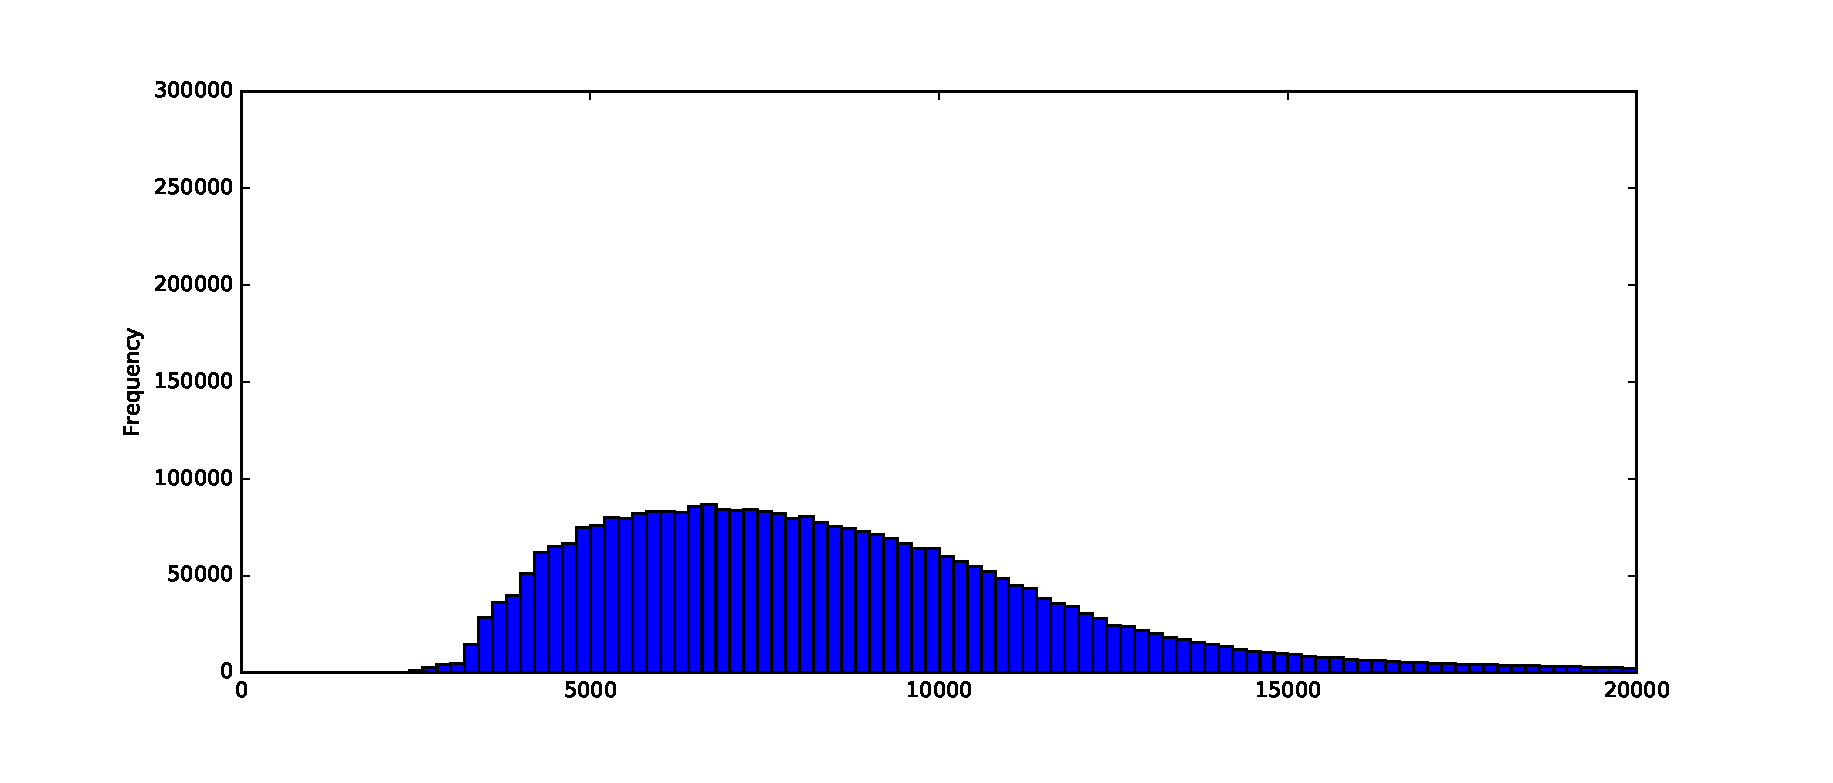
\includegraphics[width=\textwidth]{eps/spark_join_2node_th_max_hist}

       \caption{Spark, 2-node, max  throughput}
                       \label{fig_spark_join_2node_max}
   \end{subfigure}%
   \begin{subfigure}[b]{0.3\textwidth}
       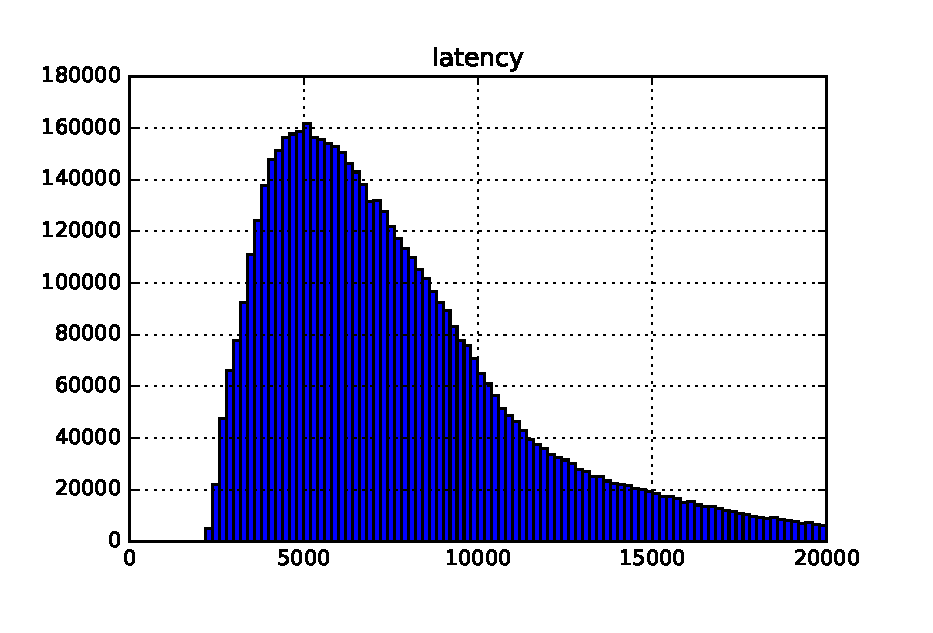
\includegraphics[width=\textwidth]{eps/spark_join_4node_th_max_hist}

       \caption{Spark, 4-node, max  throughput }
                       \label{fig_spark_join_4node_max}
   \end{subfigure}%
   \begin{subfigure}[b]{0.3\textwidth}
       \includegraphics[width=\textwidth]{eps/spark_join_8node_th_max_hist}

       \caption{Spark, 8-node, max  throughput }
                       \label{fig_spark_join_8node_max}
   \end{subfigure}




   \begin{subfigure}[b]{0.3\textwidth}
       \includegraphics[width=\textwidth]{eps/flink_join_2node_th_max_hist}

       \caption{Flink, 2-node, max  throughput}
   \end{subfigure}%
   \begin{subfigure}[b]{0.3\textwidth}
       \includegraphics[width=\textwidth]{eps/flink_join_4node_th_max_hist}

       \caption{Flink, 4-node, max  throughput }
   \end{subfigure}%
   \begin{subfigure}[b]{0.3\textwidth}
       \includegraphics[width=\textwidth]{eps/flink_join_8node_th_max_hist}

       \caption{Flink, 8-node, max  throughput }
   \end{subfigure}
   
   
   
   
      \begin{subfigure}[b]{0.3\textwidth}
       \includegraphics[width=\textwidth]{eps/spark_join_2node_th_90_hist}

       \caption{Spark, 2-node,  90\%-throughput}
   \end{subfigure}%
   \begin{subfigure}[b]{0.3\textwidth}
       \includegraphics[width=\textwidth]{eps/spark_join_4node_th_90_hist}

       \caption{Spark, 4-node,  90\%-throughput }
   \end{subfigure}%
   \begin{subfigure}[b]{0.3\textwidth}
       \includegraphics[width=\textwidth]{eps/spark_join_8node_th_90_hist}

       \caption{Spark, 8-node,  90\%-throughput }
   \end{subfigure}




   \begin{subfigure}[b]{0.3\textwidth}
       \includegraphics[width=\textwidth]{eps/flink_join_2node_th_90_hist}

       \caption{Flink, 2-node,  90\%-throughput}
   \end{subfigure}%
   \begin{subfigure}[b]{0.3\textwidth}
       \includegraphics[width=\textwidth]{eps/flink_join_4node_th_90_hist}

       \caption{Flink, 4-node,  90\%-throughput }
   \end{subfigure}%
   \begin{subfigure}[b]{0.3\textwidth}
       \includegraphics[width=\textwidth]{eps/flink_join_8node_th_90_hist}

       \caption{Flink, 8-node,  90\%-throughput }
   \end{subfigure}

        \caption{Windowed join latency distributions in histogram.}
                \label{fig_hist_join}
\end{figure*}








\begin{figure*}
    \centering
   \begin{subfigure}[b]{0.3\textwidth}
       \includegraphics[width=\textwidth]{eps/spark_join_2node_th_max_ts}

       \caption{Spark, 2-node, max  throughput}
       \label{fig_spark_join_2node_th_max_ts}
   \end{subfigure}%
   \begin{subfigure}[b]{0.3\textwidth}
       \includegraphics[width=\textwidth]{eps/spark_join_4node_th_max_ts}

       \caption{Spark, 4-node, max  throughput }
              \label{fig_spark_join_4node_th_max_ts}
   \end{subfigure}%
   \begin{subfigure}[b]{0.3\textwidth}
       \includegraphics[width=\textwidth]{eps/spark_join_8node_th_max_ts}

       \caption{Spark, 8-node, max  throughput }
              \label{fig_spark_join_8node_th_max_ts}
   \end{subfigure}




   \begin{subfigure}[b]{0.3\textwidth}
       \includegraphics[width=\textwidth]{eps/flink_join_2node_th_max_ts}

       \caption{Flink, 2-node, max  throughput}
   \end{subfigure}%
   \begin{subfigure}[b]{0.3\textwidth}
       \includegraphics[width=\textwidth]{eps/flink_join_4node_th_max_ts}

       \caption{Flink, 4-node, max  throughput }
   \end{subfigure}%
   \begin{subfigure}[b]{0.3\textwidth}
       \includegraphics[width=\textwidth]{eps/flink_join_8node_th_max_ts}

       \caption{Flink, 8-node, max  throughput }
   \end{subfigure}
   
   
   
   
      \begin{subfigure}[b]{0.3\textwidth}
       \includegraphics[width=\textwidth]{eps/spark_join_2node_th_90_ts}

       \caption{Spark, 2-node,  90\%-throughput}
   \end{subfigure}%
   \begin{subfigure}[b]{0.3\textwidth}
       \includegraphics[width=\textwidth]{eps/spark_join_4node_th_90_ts}

       \caption{Spark, 4-node,  90\%-throughput }
   \end{subfigure}%
   \begin{subfigure}[b]{0.3\textwidth}
       \includegraphics[width=\textwidth]{eps/spark_join_8node_th_90_ts}

       \caption{Spark, 8-node,  90\%-throughput }
   \end{subfigure}




   \begin{subfigure}[b]{0.3\textwidth}
       \includegraphics[width=\textwidth]{eps/flink_join_2node_th_90_ts}

       \caption{Flink, 2-node,  90\%-throughput}
   \end{subfigure}
   ~ 
   \begin{subfigure}[b]{0.3\textwidth}
       \includegraphics[width=\textwidth]{eps/flink_join_4node_th_90_ts}

       \caption{Flink, 4-node,  90\%-throughput }
   \end{subfigure}
   ~ 
   \begin{subfigure}[b]{0.3\textwidth}
       \includegraphics[width=\textwidth]{eps/flink_join_8node_th_90_ts}

       \caption{Flink, 8-node,  90\%-throughput }
   \end{subfigure}

        \caption{Windowed join latency distributions in time series}
                \label{fig_ts_join}
\end{figure*}













Figures  \ref{fig_hist_join} and \ref{fig_ts_join} show the latency for the windowed joins case as  histogram and time-series .  In contrast to windowed aggregations, we see the substantial fluctuations in Spark in Figures \ref{fig_spark_join_2node_th_max_ts}, \ref{fig_spark_join_4node_th_max_ts} and \ref{fig_spark_join_8node_th_max_ts}.
Also we can see a significant latency increase in Flink when compared to windowed aggregation experiments. The reason is that windowed joins are   more expensive than windowed aggregations. However, the spikes are significantly reduced with 90\% workload.  


\subsection{Discussion}

%Given the benchmarking system and the output, we derive  conclusions out of experimental results. In general there is no single winner and each system is good for specific use-case as all three SUTs have large communities and considerable amount of support in industry. However, it is important to notice the key points derived out of this experiments. 

% \todo[inline]{Please reduce the generic sentences, this is obvious=>fixed}
 
Throughout the experiments, we notice that Storm has a comparable performance  to Spark. Storm could provide more high level abstractions  with transparent on/of-heap memory management in the engine. We can see from resource utilization graphs that the usage of low level APIs results to high CPU and network usage in system.  Although Trident is a high level abstraction on top of Storm, its efficiency is much lower than Storm and with large batch sizes, it produces wrong results. Moreover, Storm's backpressure mechanism needs further enhancements as it can stall the topology with high throughputs.

Although Spark performs worse than Storm in terms of throughput, its high level APIs and advanced and the dynamic memory management is better than Storm and competitive with Flink. One downside of Spark is that it schedules one job at a time. So there is only one active job at a time.  Although there is an experimental feature to start multiple mini-batch jobs at a time, this can lead to unexpected sharing of resources. Moreover, Spark's backpressure mechanism was significantly improved  in recent releases but there is still need for further improvement. 

Flink performs best in throughput and in $avg$ latency. However, its $max$ latency is worse in comparison to other systems. Flink could add a dynamic buffer management feature to change the size of buffers at runtime to reduce the latency. We noticed the performance of Flink's backpressure to be the best because of its robustness and its low overhead.


There is no single winner according to the experimental results. Storm's and Spark's throughputs in windowed aggregations are comparable but in terms of $avg$ latency Storm is better. So if a user needs to use lower level APIs to implement custom business logic, then Storm is the best engine for windowed aggregation. However, Spark reduces latency when scaling out. So, when working with very large clusters Spark can outperform Storm. Flink on the other hand, provides the highest throughput and the lowest  $avg$ latency with its transparent and high level APIs. However, its  high $max$ latency is a limitation when compared to other systems.  







%\todo[inline]{This is still a bit unstructured, maybe you can get the overall comparison in order, e.g., per system and then total}































%    \begin{table}
        \begin{tabular}{lllll}\toprule
            &\textbf{2 Node}  & \textbf{4 Node} & \textbf{8 Node}\\\midrule
            Storm & 408K & 696K & XXX  \\
            Spark & 379K & 642K & 912K  \\
            Flink & 1230K & *1260K & *1260K \\
            \\\bottomrule
        \end{tabular}
        \caption{Sustainable throughput for windowed aggregations}\label{Tab1}
    \end{table} 



    \begin{table}
        \begin{tabular}{lllll}\toprule
            &\textbf{2 Node}  & \textbf{4 Node} & \textbf{8 Node}\\\midrule
            Storm & 1424ms & 2043ms & XXX \\
            Storm(90\%) & 1109ms & 1669ms & XXX \\
            Spark & 3759ms & 4138ms & 3152ms\\
            Spark(90\%) & 3418ms & 2846ms & 2798ms\\
            Flink & 576ms & 259ms & 243ms \\
            Flink(90\%) & 299ms & -  & - \\
            \\\bottomrule
        \end{tabular}
        \caption{Average Latency for windowed aggregations}\label{Tab1}
    \end{table} 


    \begin{table}
        \begin{tabular}{lllll}\toprule
            &\textbf{2 Node}  & \textbf{4 Node} & \textbf{8 Node}\\\midrule
            Storm & xxx & xxx & XXX  \\
            Spark & 365K & 632K & 947K  \\
            Flink & 851K & 1128K & *1260K \\
            \\\bottomrule
        \end{tabular}
        \caption{Sustainable throughput for windowed joins}\label{Tab1}
    \end{table} 



    \begin{table}
        \begin{tabular}{lllll}\toprule
            &\textbf{2 Node}  & \textbf{4 Node} & \textbf{8 Node}\\\midrule
            Storm & 1424ms & 2043ms & XXX \\
            Storm(90\%) & 1109ms & 1669ms & XXX \\
            Spark & 8417ms & 7823ms & 7590ms\\
            Spark(90\%) & 7538ms & 5825ms & 6015ms\\
            Flink & 4825ms & 4255ms & *3748ms \\
            Flink(90\%) & 3872ms & 3285ms  & - \\
            \\\bottomrule
        \end{tabular}
        \caption{Average Latency for windowed joins}\label{Tab1}
    \end{table} 

%\begin{figure*}
    \centering
    \begin{subfigure}[b]{0.3\textwidth}
        \includegraphics[width=\textwidth]{eps/storm_agg_2node_th_max_hist}
         \includegraphics[width=\textwidth]{eps/storm_agg_2node_th_max_ts}

        \caption{2 Node latency with max throughput}
    \end{subfigure}
    ~ 
    \begin{subfigure}[b]{0.3\textwidth}
        \includegraphics[width=\textwidth]{eps/storm_agg_4node_th_max_hist}
         \includegraphics[width=\textwidth]{eps/storm_agg_4node_th_max_ts}

        \caption{4 Node latency with max throughput }
    \end{subfigure}
    ~ 
    \begin{subfigure}[b]{0.3\textwidth}
        \includegraphics[width=\textwidth]{eps/storm_agg_8node_th_max_hist}
         \includegraphics[width=\textwidth]{eps/storm_agg_8node_th_max_ts}

        \caption{8 Node latency with max throughput }
    \end{subfigure}




    \begin{subfigure}[b]{0.3\textwidth}
        \includegraphics[width=\textwidth]{eps/storm_agg_2node_th_90_hist}
         \includegraphics[width=\textwidth]{eps/storm_agg_2node_th_90_ts}

        \caption{2 Node latency with 90\% throughput }
    \end{subfigure}
    ~ 
    \begin{subfigure}[b]{0.3\textwidth}
        \includegraphics[width=\textwidth]{eps/storm_agg_4node_th_90_hist}
         \includegraphics[width=\textwidth]{eps/storm_agg_4node_th_90_ts}

        \caption{4 Node latency with 90\% throughput }
    \end{subfigure}
    ~ 
    \begin{subfigure}[b]{0.3\textwidth}
        \includegraphics[width=\textwidth]{eps/storm_agg_8node_th_90_hist}
         \includegraphics[width=\textwidth]{eps/storm_agg_8node_th_90_ts}

        \caption{4 Node latency with 90\% throughput }
    \end{subfigure}




        \caption{Latency of windowed aggregations for Storm}
\end{figure*}
%\include{images/tex/spark_agg}
%\begin{figure*}
    \centering
    \begin{subfigure}[b]{0.3\textwidth}
        \includegraphics[width=\textwidth]{eps/flink_agg_2node_th_max_hist}
         \includegraphics[width=\textwidth]{eps/flink_agg_2node_th_max_ts}

        \caption{2 Node latency with maximum throughput}
    \end{subfigure}
    ~ 
    \begin{subfigure}[b]{0.3\textwidth}
        \includegraphics[width=\textwidth]{eps/flink_agg_4node_th_max_hist}
         \includegraphics[width=\textwidth]{eps/flink_agg_4node_th_max_ts}

        \caption{4 Node latency with network bounded throughput }
    \end{subfigure}
   ~
    \begin{subfigure}[b]{0.3\textwidth}
        \includegraphics[width=\textwidth]{eps/flink_agg_8node_th_max_hist}
         \includegraphics[width=\textwidth]{eps/flink_agg_8node_th_max_ts}

        \caption{8 Node latency with network bounded throughput }
    \end{subfigure}
    ~ 
    \begin{subfigure}[b]{0.3\textwidth}
        \includegraphics[width=\textwidth]{eps/flink_agg_2node_th_90_hist}
         \includegraphics[width=\textwidth]{eps/flink_agg_2node_th_90_ts}

        \caption{2 Node latency with 90\% throughput }
    \end{subfigure}
    ~ 
    \begin{subfigure}[b]{0.3\textwidth}
        \includegraphics[width=\textwidth]{eps/flink_agg_4node_th_90_hist}
         \includegraphics[width=\textwidth]{eps/flink_agg_4node_th_90_ts}

        \caption{2 Node latency with 90\% throughput }
    \end{subfigure}
    ~ 
    \begin{subfigure}[b]{0.3\textwidth}
        \includegraphics[width=\textwidth]{eps/flink_agg_8node_th_90_hist}
         \includegraphics[width=\textwidth]{eps/flink_agg_8node_th_90_ts}

        \caption{2 Node latency with 90\% throughput }
    \end{subfigure}




        \caption{Latency of windowed aggregations for Flink}
\end{figure*}
%\include{images/tex/spark_join}
%\include{images/tex/flink_join}












\section{Conclusions}
\label{conc}

Responding to an increasing use of real time data processing in industry and in academia, we build a novel framework for benchmarking stream data processing engines. We identify the current challenges in this area and build our solution to solve them. First, we give the  definition of latency of a stateful operator and a methodology to measure it. The solution is lightweight and does not require the use of additional systems. Second, we completely separate the systems under test from the driver.  Third, we introduce a simple and novel technique to conduct  experiments with the highest sustainable workloads. %Finally, we achieve the above contributions with simple design. 
We conduct extensive experiments with the three major distributed, open source stream processing engines - Apache Storm, Apache Spark, and Apache Flink. In the experiments, we can see that there is no single winner.  Each system has specific advantages and challenges. Thus, users need to take use-case requirements into account when choosing the right system. 
We are currently extending the benchmarking framework to handle several other metrics like query throughput. In addition, we are developing a generic interface that the users can plug into any stream data processing system, in order to facilitate and simplify benchmarking.
%\todo[inline]{The conclusion should include the contributions and the take home message (which is missing currently). Also we need some future work.}
\section{Acknowledgments}
The authors would like to acknowledge the invaluable help of Rovio Entertainment in providing the use-cases. This work has been supported by the European Commission through Proteus (ref. 687691) and Streamline (ref. 688191) and by the German Ministry for Education and Research as Berlin Big Data Center BBDC (funding mark 01IS14013A). 
















% ensure same length columns on last page (might need two sub-sequent latex runs)
\balance

% The following two commands are all you need in the
% initial runs of your .tex file to
% produce the bibliography for the citations in your paper.
\bibliographystyle{abbrv}
\bibliography{vldb_sample}  % vldb_sample.bib is the name of the Bibliography in this case
% You must have a proper ".bib" file
%  and remember to run:
% latex bibtex latex latex
% to resolve all references


%APPENDIX is optional.
% ****************** APPENDIX **************************************
% Example of an appendix; typically would start on a new page
%pagebreak






\end{document}
